\documentclass{article}
\usepackage[utf8]{inputenc}
\usepackage{lmodern}
\usepackage{blindtext}
\usepackage{amsmath}
\usepackage[a4paper, inner=1.7cm, outer=2.7cm, top=3cm, bottom=3cm, bindingoffset=1.2cm]{geometry}
\usepackage{tcolorbox}
\usepackage{graphicx}
\usepackage{wrapfig}
\usepackage{makecell}
\usepackage{boldline}
\usepackage{float}
\usepackage{tabularx}
\usepackage[table]{colortbl}
\usepackage[english]{babel}
\usepackage{amsthm}
\usepackage{hyperref}

\newtheorem*{invariant}{Invariant}

\renewcommand\theadalign{bc}
\renewcommand\theadfont{\bfseries}
\renewcommand\theadgape{\Gape[4pt]}
\renewcommand\cellgape{\Gape[4pt]}

\begin{document}

\title{\textbf{Chicken Bonds: Self-Bootstrapping Liquidity}}
\author{Liquity Team}
\date{July 7, 2021}

\maketitle

\section*{Abstract}
Chicken Bonds are a novel product for DAOs/projects to bootstrap protocol owned liquidity (POL) at no cost while boosting yield opportunities for their end users. The yield amplification is achieved by directing additional yield from POL and users bonding underlying tokens (TKN) to newly issued “boosted” tokens (bTKN). 

Acting as an autonomous self-bootstrapping treasury, the protocol is powered by an innovative bonding mechanism: users may deposit TKN in exchange for an accruing balance of bTKN. At any time, bond holders can either retrieve their principal foregoing the accrued amount (“chicken out”) or trade it in for the accrued bTKN (“chicken in”).

The TKN acquired by the system backs the bTKN supply: while a portion of the TKN in the treasury is directly redeemable by bTKN holders, another portion is contributing permanently to the redeemable value through its yield. Along with the yield retained from pending bonds, the bTKN benefits from a rapidly rising price floor,  making it an attractive investment.

Chicken Bonds are versatile and can be used by protocols to obtain DEX liquidity or to pursue sophisticated liquidity management strategies including algorithmic market operators (AMOs). An interesting use case involves bonding LP tokens.

\tableofcontents

\section{Introduction}
DeFi summer 2020 has led to an abundance of DeFi projects, making it increasingly competitive to maintain liquid markets for new protocol tokens. Many projects have faced excessive costs of obtaining liquidity from providers looking for the best short-term yield farming opportunities. Such capital lacks stickiness and moves on as higher-yield options become available. Protocols are thus only renting temporary liquidity from users at high costs.

More recently, DeFi 2.0 protocols such as Olympus Pro, Ondo and Tokemak have started offering alternative ways to acquire liquidity, which are more similar to leasing or buying. While tackling the issue of stickiness, they are still costly and may not be affordable for all projects.

Chicken Bonds is a major innovation in liquidity acquisition technology and works with any underlying token (TKN) that can be used to earn yield, e.g. in a DEX, a lending protocol or through native staking.

The system offers strong benefits to DeFi protocols and bond holders, while minimizing risk:

\begin{itemize}
    \item \textit{Cost-free liquidity accumulation for projects}. Rather than purchasing or renting liquidity, the system freely acquires treasury assets over time in a self-bootstrapping manner. Liquidity acquisition is incentivized by the amplified yields that are attainable by bond holders, enabled by the novel bonding dynamics.
    \item \textit{Risk-free and flexible bonding for users}. Bond holders may “chicken out” and withdraw their deposited principal at any time, in lieu of converting it to “boosted” tokens (bTKN). Therefore bonding is fully reversible and bond holders are not locked into any commitment to the protocol. Furthermore, bonds are represented as NFTs and can thus be sold on the secondary market, which can be attractive for bonds that have accumulated a significant amount of bTKN.
    \item \textit{System stability and resilience}. The Chicken Bonds derivative token bTKN has a hard price floor supported by a direct redemption mechanism. Most of the time, bTKN will in fact trade at a premium above this price floor due to amplified (“boosted”) yield earned by the underlying liquidity. Though the premium may vary, the bonding rules guarantee that the price floor can only increase over time. As such, the Chicken Bonds boosted token does not suffer from the high volatility and strong reflexivity inherent to secondary tokens issued by other bonding protocols
\end{itemize}

\section{Treasury}
The protocol operates a \textit{Treasury R} consisting of three logical parts (“buckets”):  \textit{Pending Bucket}, \textit{Reserve Bucket} and \textit{Permanent Bucket}.

Each bucket contains a certain quantity of TKN or other assets whose value can be readily expressed in TKN. We suppose that the assets in the buckets can be invested in a third-party protocol (e.g. staked natively or deposited to a DEX) to generate yield while being withdrawable at any time. 

The current state of the Treasury can thus be described by the following tuple:

\begin{equation}
  \label{eq:treasury}
    R:=(q_p, q_r, q_d, r_p, r_r, r_d)
\end{equation}

where $q_p$, $q_r$ and $q_d$ stand for the quantities held by the respective buckets, and $r_p$, $r_r$, $r_d$ for their rates of return. Note that the buckets as logical quantities do not need to correspond to the physical investment vehicles. A bucket may invest its funds to multiple investment vehicles, and several buckets may use the same venue earning the same rate of return.

The buckets are used as follows:
\begin{itemize}
    \item \textit{Pending Bucket.} Contains the TKN bonded by users that are still active bond holders, i.e. whose deposits haven’t been acquired by the protocol yet. Since bond holders may withdraw their bonded TKN at will (see \ref{sec:chicken-out} “chicken out“), their deposits are considered as pending. The yield earned by the Pending Bucket is credited to the Reserve Bucket.
    \item \textit{Reserve Bucket.} Contains a portion of the TKN relinquished by former bond holders after a "chicken in" event (see \ref{sec:chicken-in}) as well as the yield of the Pending and the Permanent Buckets. The Reserve Bucket directly backs the bTKN supply through the redemption mechanism (see \ref{sec:redemption}).
    \item \textit{Permanent Bucket.} Contains the other portion of the TKN relinquished by former bond holders. The yield earned by the Permanent Bucket is credited to the Reserve Bucket.
\end{itemize}

Having a Permanent Bucket may turn out as unnecessary or even detrimental for some use cases. As an alternative, the protocol can thus be set up without a Permanent Bucket (see \ref{sec:two-bucket}).

\subsection{Yield Amplification and Reinvestment}
Given that the Reserve Bucket earns a return not only on its own assets, but additionally receives the returns from the Pending and the Permanent Buckets, it achieves an amplified return $r_r^\star > r_r$ on the amount $q_r$. We call this useful property \textit{yield amplification}.

As the protocol doesn't distribute any yields, but reinvests them inside the Reserve Bucket, the value of the Reserve Bucket will grow over time even without the inflow of new capital. Due to the yield amplification, the Reserve Bucket grows faster than if the same funds were invested regularly with a (compounding) rate of return $r_r$.

\subsection{Reserve Bucket backing the Boosted Token}
The protocol maintains a supply $S$ of a \textit{Boosted Token} (bTKN) according to preset rules for minting and burning. The bTKN supply is directly backed by the Reserve Bucket, i.e. it can be redeemed against a pro rata share of the assets (usually TKN) held therein (see \ref{sec:chicken-out}).

We call the amount of TKN for which each bTKN can be redeemed for the \textit{redemption price} $p_r$. The redemption price  corresponds to the \textit{backing ratio} and is defined as $\frac{q_r}{S}$. It is subject to the following invariant:

\begin{invariant}[Redemption price never decreases]
The protocol ensures that the redemption price $p_r$ (backing ratio) can only ever increase, but never decrease.
\end{invariant}

\section{User interactions}

Users can interact with the protocol in the followings ways:
\begin{itemize}
    \item \textit{Bonding}. Users can bond TKN in order to earn bTKN.
    \item \textit{Redemption}. Users can redeem bTKN for TKN.
\end{itemize}

\subsection{Bonding}
Bonding is the main use case that allows the system to build up its treasury by incentivizing users through the issuance of a  \textit{Boosted Token}, the bTKN. 

Users can bond any amount $b$ of TKN at any time in exchange for a position called \textit{Chicken Bond}, represented by an NFT. The bonded TKN is added to the \textit{Pending Bucket} where it earns a yield for the system's Treasury.

A Chicken Bond accrues a virtual balance $s(t)$ of bTKN over time, according to a curve that asymptotically approaches a "cap" ensuring the invariant of a never decreasing redemption price. 

The protocol may exclude a portion of the bonded amount from accruing bTKN, and divert it as an incentive to LPs of a bTKN/TKN exchange pair when the user opts to chicken in (see \ref{sec:chicken-in}). We therefore call this portion the chicken-in fee (see \ref{sec:chicken-in-fee}).

The accrual curve can be of the form 

\begin{equation}
  \label{eq:accrual}
    s(t) := \frac{b}{p_r} \cdot \frac{t}{t+\alpha}
\end{equation}

\begin{figure}
    \centering
    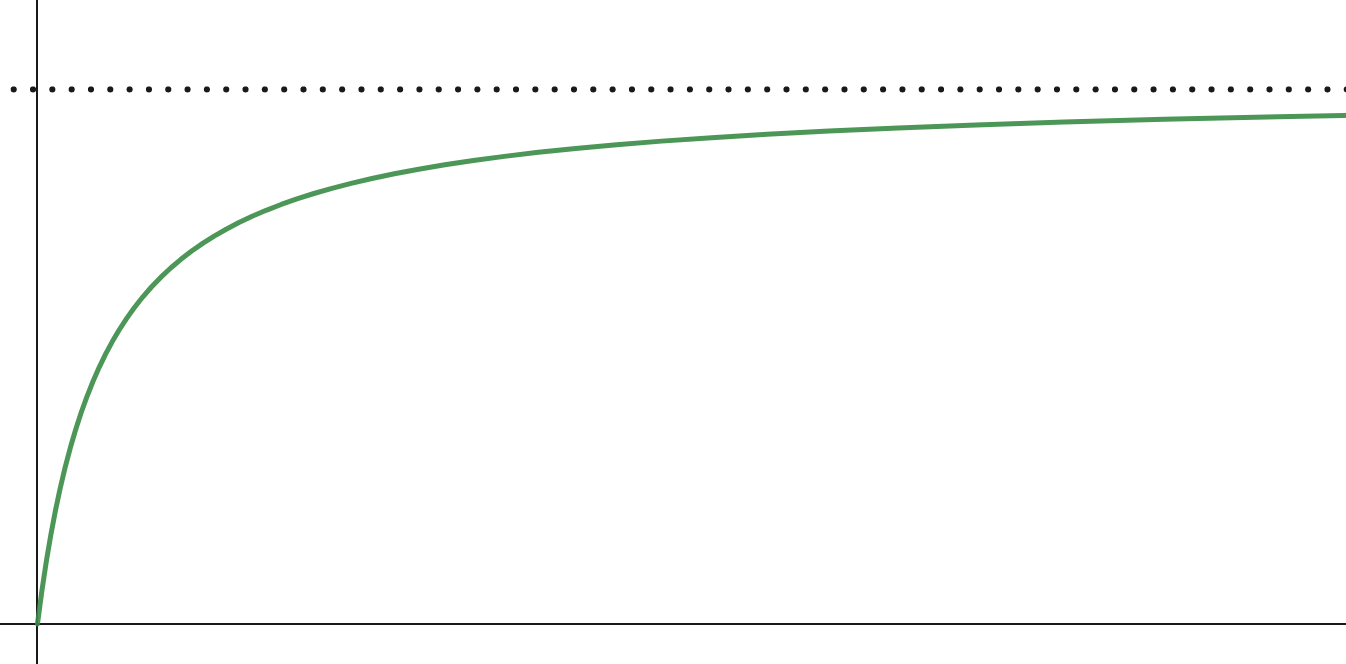
\includegraphics[width=0.5\linewidth]{./ChickenBonds_Whitepaper_accrualcurve.png}
\end{figure}

$\alpha$ parametrizes the slope of the curve and could be automatically adjusted by the protocol in order to control the speed of the value accrual which depends on the evolving price premium (see \ref{sec:adjustment}).

We call the fraction $\frac{b}{p_r}$ the cap $c$ which corresponds to the amount of bTKN that could be minted by the protocol such that the redemption price would be kept constant if $b$ was entirely added to the Reserve Bucket. Therefore, the ratio between the cap and the bond corresponds to the ratio between the bTKN supply and the Reserve Bucket. Thus, we have

\begin{equation}
  \label{eq:cap-bond-ratio}
    \frac{c}{b} = \frac{S}{q_r}
\end{equation}   

The owner of a \textit{Chicken Bond} can exit their position any time by choosing either of the following options:

\begin{itemize}
    \item \textit{Chicken out}. Retrieve the principal foregoing the accrued bTKN.
    \item \textit{Chicken in}. Obtain the accrued bTKN foregoing the bonded TKN.
\end{itemize}

\begin{figure}[ht]
    \centering
    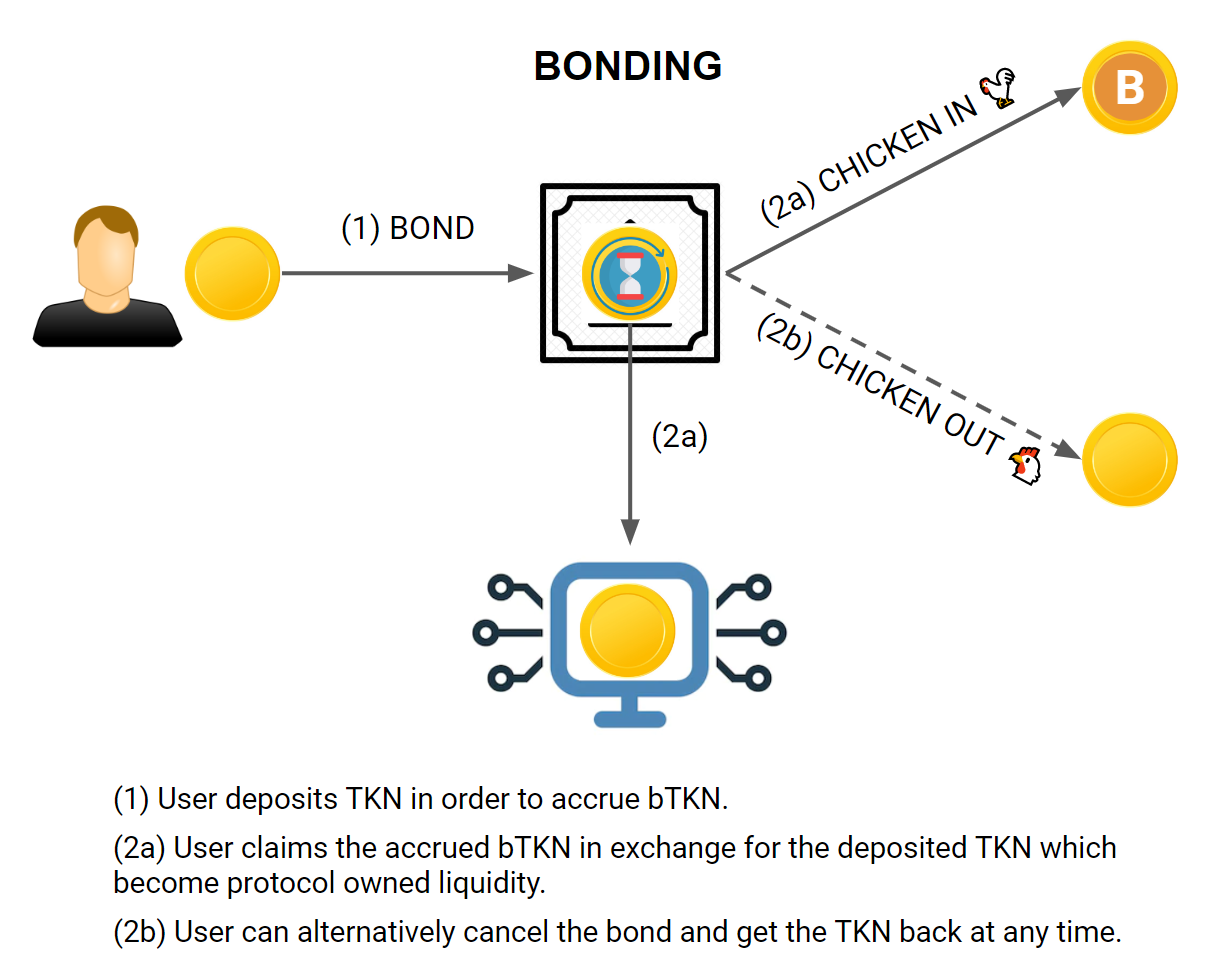
\includegraphics[width=0.5\linewidth]{./ChickenBonds_Whitepaper_ci_co.png}
\end{figure}

In both cases, the Chicken Bond NFT is burned as the bond holder’s position is closed. Depending on the option chosen, the bonded TKN is either fully paid back to the user or it transitions from the Pending Bucket to the Reserve Bucket and the Permanent Bucket according to a split calculated by the system (\ref{sec:chicken-in}). 

\subsubsection{Chicken out}
\label{sec:chicken-out}
By chickening out, the bond holder gets the entire bonded TKN back, foregoing the accrued balance of bTKN (which doesn’t get minted). The option to withdraw the principal at any time makes bonding an essentially risk-free investment where the user only incurs the opportunity costs besides smart contract risks.

Upon a chicken out event at time $t_{i+1}$ (where previous event in the system occurred at time $t_i$), the Treasury changes as follows:

\begin{equation}
  \label{eq:chicken-out-transition}
    q_p(t_{i+1}) := q_p(t_i) - b
\end{equation}

As an alternative, the bond holder may sell their NFT on the secondary market. The buyer of the NFT has the same rights against the protocol as the original bond holder.

\subsubsection{Chicken in}
\label{sec:chicken-in}
A user that chickens in loses the bonded TKN in exchange for the accrued balance of bTKN that is minted and paid out by the protocol. 

Instead of keeping the received bTKN, the user may sell it on the open market and opt to reinvest the proceeds by creating a new, typically larger bond (aka as “rebonding”, see below).

Upon a chicken in, the protocol acquires the bonded TKN which is moved from the Pending Bucket to the Reserve Bucket and the Permanent Bucket. To that end, the bonded amount $b$ is first split into two amounts $b_r$ and $b_d$ in proportion to the ratio of the currently accrued bTKN $s$ to the cap $c$:

\begin{equation}
  \label{eq:chicken-in-ba}
    b_r = \frac{s}{c} \cdot b = s \cdot p_r
\end{equation}
\begin{equation}
  \label{eq:chicken-in-bd}
    b_d = \frac{c-s}{c} \cdot b = b - s \cdot p_r
\end{equation}

The two amounts are then added to the Reserve and the Permanent Bucket, so that the Treasury transitions to the following state:

\begin{equation}
  \label{eq:chicken-in-qa}
    q_r(t_{i+1}) := q_r(t_i) + b_r = q_r(t_i) + s \cdot p_r
\end{equation}
\begin{equation}
  \label{eq:chicken-in-qd}
    q_d(t_{i+1}) := q_d(t_i) + b_d = q_d(t_i) + b - s \cdot p_r
\end{equation}
\begin{equation}
  \label{eq:chicken-in-qp}
    q_p(t_{i+1}) := q_p(t_i) - b
\end{equation}
\begin{equation}
  \label{eq:chicken-in-S}
    S(t_{i+1}) := S(t_i) + s
\end{equation}

Note that a portion of the bonded amount may be diverted as an incentive for bTKN/TKN LPs (see \ref{sec:chicken-in-fee}) instead of being split between the mentioned buckets.

\begin{figure}[ht]
    \centering
    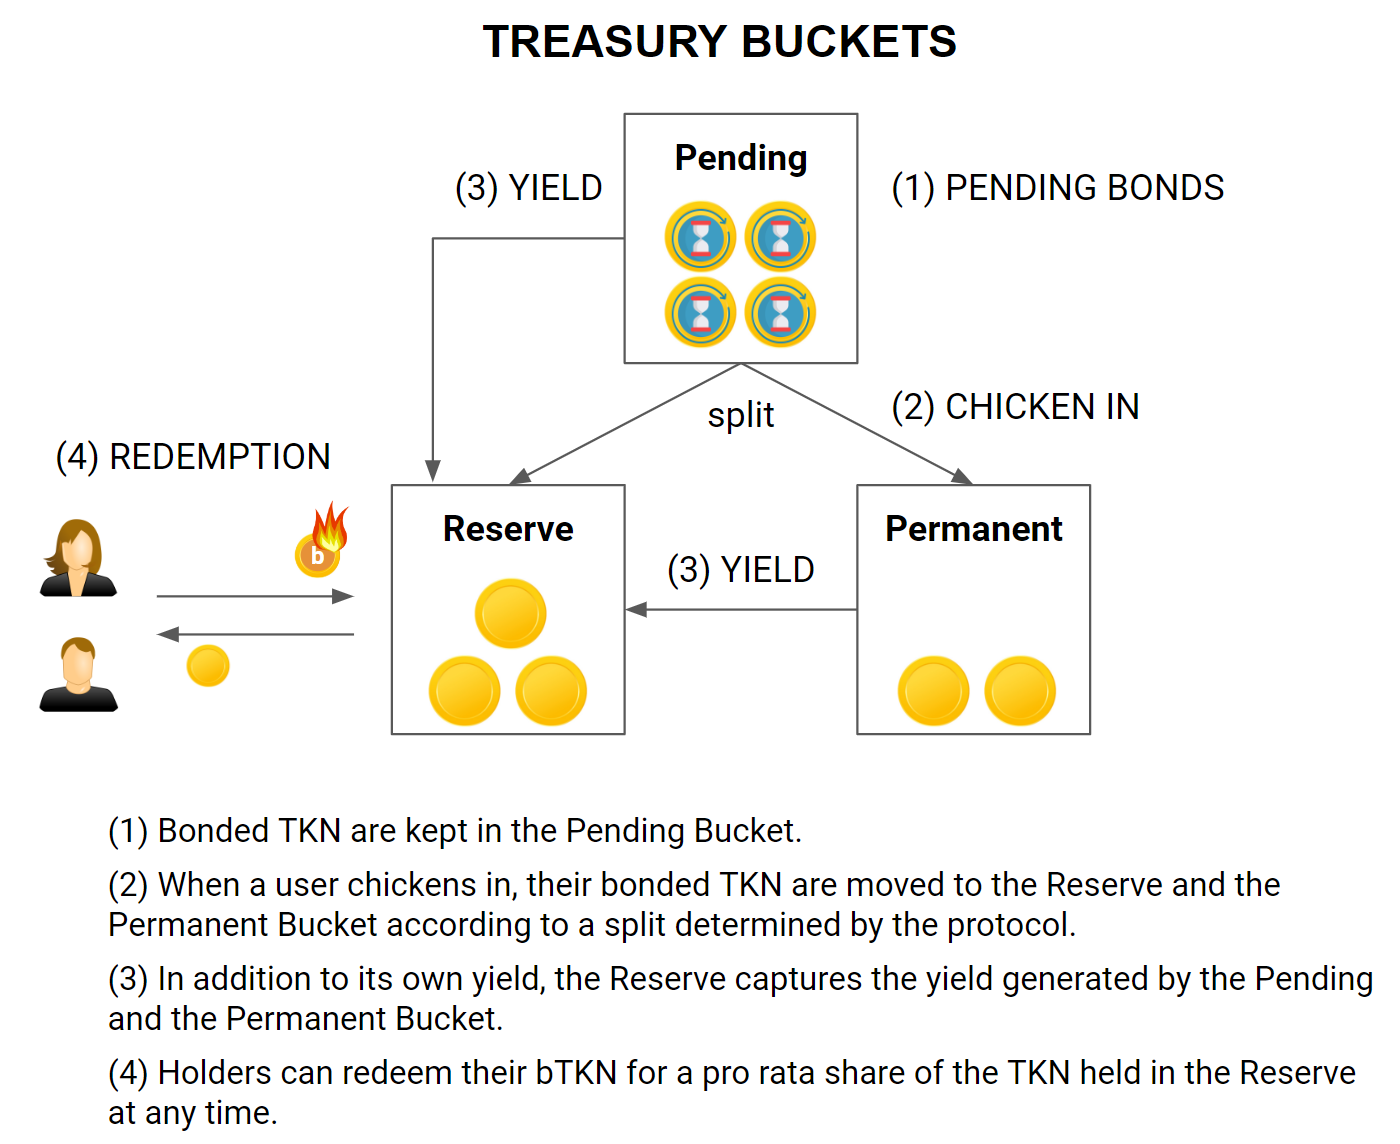
\includegraphics[width=0.5\linewidth]{./ChickenBonds_Whitepaper_treasury.png}
\end{figure}

\subsection{Redemption}
\label{sec:redemption}
At any time, a holder can redeem $n$ bTKN for $\frac{n}{S}\cdot q_r = n \cdot p_r$ TKN.
The TKN are removed from the Reserve Bucket and paid out the user, while the redeemed bTKN are burned.

The state of the Treasury changes as follows: 

\begin{equation}
  \label{eq:redemption-qa}
    q_r(t_{i+1}) := q_r(t_i) \cdot (1 - \frac{n}{S})
\end{equation}
\begin{equation}
  \label{eq:redemption-S}
    S(t_{i+1}) := S(t_i) - n
\end{equation}

To throttle the rate of redemption or counter extreme situations and black swan events, the system could charge a redemption fee (see \ref{sec:redemption-fee}).

\section{Economics of Chicken Bonds}
 \label{sec:economics}
The Boosted Token bTKN derives its value from the Reserve Bucket, as its direct backing, and the yield generated by the entire Treasury.

Since the bTKN supply is redeemable for a proportional share of the acquired TKN, the market cap of bTKN should normally be worth at least the amount of TKN kept in the Reserve Bucket. This means that the redemption price $p_r$ will act as a price floor, below which arbitrage becomes possible: people can buy bTKN for less than what they get upon redemption. Should bTKN ever drop below the redemption price, we can expect it to bounce back quickly due to the buying pressure stemming from redemptions.

In practice, we expect bTKN to trade significantly above its price floor most of the time due to the yield amplification: if we suppose that $r_r$ corresponds to the market rate (or natural rate) $r_m$, the Reserve Bucket and thus $p_r$ will grow at a higher rate than $r_m$ given the extra yield generated by the Pending and the Permanent Bucket. This increased return warrants a price premium since the market should price in the amplified growth rate by paying a higher price for bTKN than the redemption price. We call this expected market price the \textit{fair price} $p_f$ and let $\lambda = \frac{p_f}{p_r}$ denote the \textit{relative price premium} or simply \textit{premium}, i.e. the fraction between the fair price and the redemption price.

\subsection{Profitability of bonding}
Bonding is only profitable for $\lambda>1$, i.e. if $p_f>p_r$. In that case, we can easily calculate the break even point which is reached when $p_f \cdot s(t)>b$, i.e.
\begin{equation}
  \label{eq:break_even_0}
\frac{p_f}{p_r}\frac{t}{t+\alpha} > 1
\end{equation}

Using $\lambda$:

\begin{equation}
  \label{eq:break_even_0}
\lambda\frac{t}{t+\alpha} > 1
\end{equation}

We can then solve for $t$ and write the break even point in terms of $\lambda$:

\begin{equation}
  \label{eq:break_even_2}
t > \frac{\alpha}{\lambda-1}
\end{equation}

The actual rate of return from bonding depends on $\lambda$ and the shape (steepness) of the accrual curve $s(t)$ given by the parameter $\alpha$.

\subsection{Optimal rebonding strategy}
  \label{sec:rebonding_strategy}
When people bond, they accrue a bTKN balance which they can claim by giving up the TKN amount they deposited at bond creation. Clearly then, the system doesn't auto-compound the accrued profits from bonding. In order to benefit from a compounding effect, bond holders can chicken in, sell their received bTKN for TKN and reinvest the TKN to create a new, larger bond, and repeat that process over and over again.

\begin{figure}[ht]
    \centering
    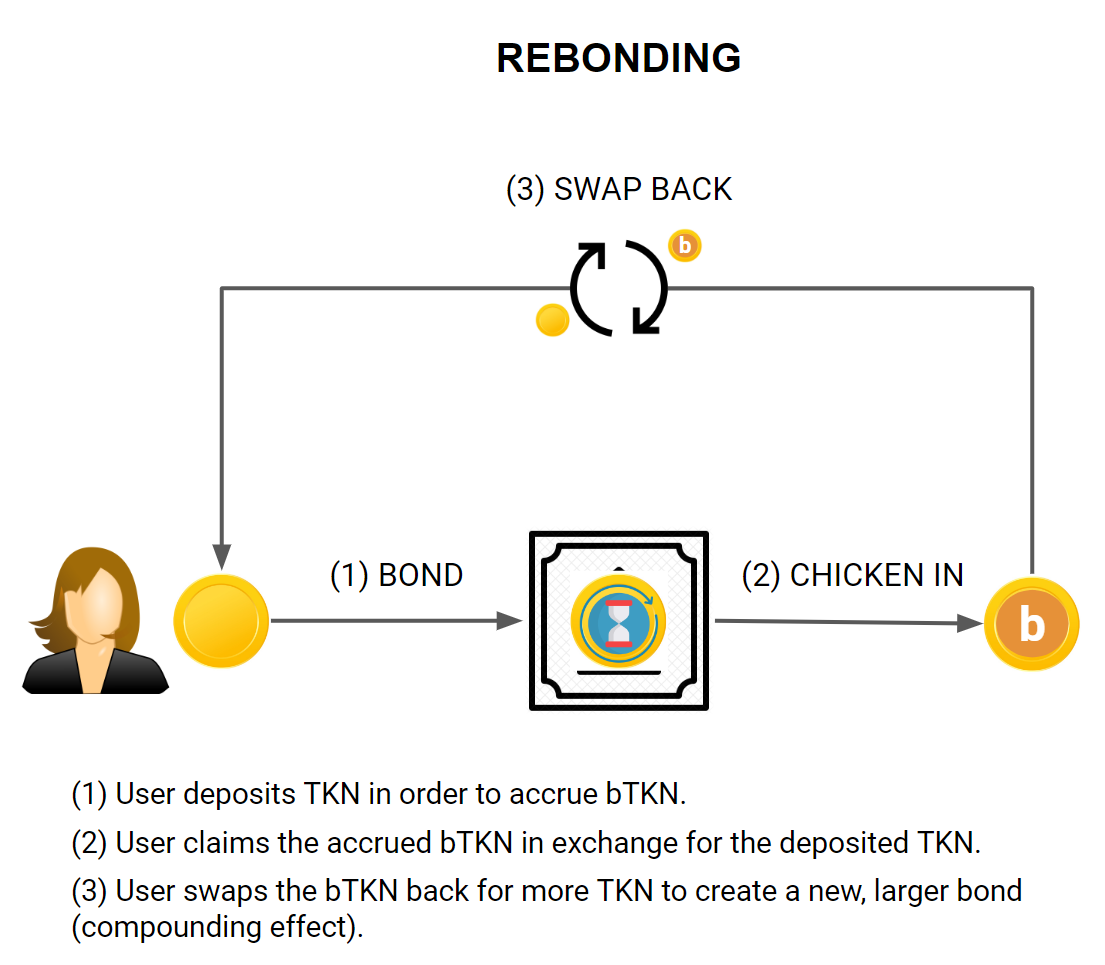
\includegraphics[width=0.5\linewidth]{./ChickenBonds_Whitepaper_rebonding_graphic.png}
\end{figure}

In the following derivation, we analyze the optimal rebonding strategy for users with a long-term time horizon by deriving a time period $T_{opt}$ which maximizes the profitability of (regular) rebonding for a given system configuration.

\subsubsection{Optimal rebonding time}
  \label{sec:T_OP}
We assume $b$ and $\lambda$ to be constant for simplicity. The impact of $\lambda$ on $T_{opt}$ and thus the accuracy of the simplification depends on the volatility of $\lambda$ and the length of the $T_{opt}$ period, which can be tuned by the controller to be relatively short, limiting the impact of the volatility. As the system matures, the yield amplification will tend to decline due to the perpetual growth of the Reserve Bucket relative to the two other buckets, which cannot sustainably grow at the same rate in the long run. With a decreasing relative size of the Permanent and Pending Buckets, their volatility should become less impactful for the fair price, making the simplification more accurate over time (at least based on the naive fair price formula, see \ref{sec:naive_approach}). The assumption may be unrealistic for the early growth phase though.

Before deriving the optimal rebonding time, we start by comparing the final value of a user's bond (expressed in TKN) after a time period $T$ without rebonding (denoted by $f$) with the final value of a bond that is rebonded at time $t<T$ (denoted by $f_r$).

\paragraph{No rebonding}
We multiply the accrued bTKN tokens from equation \ref{eq:accrual} by the market price which we assume is equal to the fair price $p_f$:

\begin{equation}
  \label{eq:o-s}
f = p_f\frac{b}{p_r}\frac{T}{T+\alpha}
\end{equation}

\paragraph{With rebonding}
At time $t$, when the user chickens in and rebonds, the new bond amount $b'$ will be:
\begin{equation}
b'= p_f\frac{b}{p_r}\frac{t}{t+\alpha}
\end{equation}

From that point until time T, there is a period of length $T-t$, during which the value of the bond will be:
\begin{equation}
f_r = p_f\frac{b'}{p_r}\frac{T-t}{T-t+\alpha}
\end{equation}

So finally we have
\begin{equation}
  \label{eq:o-r}
f_r = b\left(\frac{p_f}{p_r}\right)^2\frac{t}{t+\alpha}\frac{T-t}{T-t+\alpha}
\end{equation}

Now we can generalize this approach to $n$ regular rebonding events. We set $t=\frac{T}{n}$, and express the resulting bond value (measured in TKN) for a given rebonding period $t$ with $f_r(n)$ (note that the final period after the last rebonding event is also $\frac{T}{n}$).

\[
f_r(n) = b \left(\frac{p_f}{p_r}\right)^n \left(\frac{\frac{T}{n}}{\frac{T}{n}+\alpha}\right)^{n-1} \frac{\frac{T}{n}}{\frac{T}{n}+\alpha}
\]

\[
f_r(n) = b \left(\frac{p_f}{p_r}\right)^n \left(\frac{\frac{T}{n}}{\frac{T}{n}+\alpha}\right)^{n}
\]

\[
f_r(n) = b \left(\frac{p_f}{p_r}\right)^n \left(\frac{T}{T + n\alpha}\right)^{n}
\]

\begin{equation}
  \label{eq:n-rebond_1}
f_r(n) = b \left(\frac{p_f}{p_r} \frac{T}{T+n \alpha} \right)^{n}
\end{equation}

To find the maximum value of $f_r(n)$, we take its derivative with respect to $n$ (and we extend the domain from natural to real numbers):
\[
\begin{split}
  f_r'(n) &= b \left(\frac{p_f}{p_r} \frac{T}{T+n\alpha}\right)^n \left(\ln\left(\frac{p_f}{p_r} \frac{T}{T+n\alpha}\right) - n \frac{\frac{p_f}{p_r} \frac{\alpha T}{(T+n\alpha)^2}}{\frac{p_f}{p_r} \frac{T}{T+n\alpha}}\right) \\
  &= b \left(\frac{p_f}{p_r} \frac{T}{T+n\alpha}\right)^n \left(\ln\left(\frac{p_f}{p_r} \frac{T}{T+n\alpha}\right) - \frac{n\alpha}{T+n\alpha}\right)
\end{split}
\]

Then equating it to zero:

\[
f_r'(n) = 0 \iff \ln\left(\frac{p_f}{p_r} \frac{T}{T+n\alpha}\right) = \frac{n\alpha}{T+n\alpha}
\]

\[
\frac{p_f}{p_r} \frac{T}{T+n\alpha} = e^{\frac{n\alpha}{T+n\alpha}}
\]

Dividing both sides by $e$:

\[
\frac{p_f}{e p_r} \frac{T}{T+n\alpha} = e^{\frac{n\alpha}{T+n\alpha} - 1}
\]

\[
\frac{p_f}{e p_r} \frac{T}{T+n\alpha} = e^{\frac{-T}{T+n\alpha}}
\]

\[
\frac{T}{T+n\alpha} e^{\frac{T}{T+n\alpha}} = \frac{p_f}{e p_r} 
\]

This has the form $z e^z = w$, i.e. it is a Lambert W function: \url{https://en.wikipedia.org/wiki/Lambert_W_function}, so:

\[
\frac{T}{T+n\alpha} = W\left(\frac{p_f}{e p_r} \right)
\]

\[
1 + \frac{n\alpha}{T} = \frac{1}{W\left(\frac{p_f}{e p_r} \right)}
\]

\begin{equation}
  \label{eq:opt-rebonding-n}
n = \frac{T}{\alpha} \left(\frac{1}{W\left(\frac{p_f}{e p_r} \right)} - 1\right)
\end{equation}

To find the optimal rebonding time period $T_{opt}$, we divide the total considered period $T$ by the optimal number of rebonding events $n$, and replace $n$ by the expression above (\ref{eq:opt-rebonding-n}):

\begin{equation}
  \label{eq:opt-rebonding-prices}
T_{opt} = \frac{T}{n} = \frac{\alpha W\left(\frac{e p_r}{p_f}\right)}{1 - W\left(\frac{e p_r}{p_f}\right)}
\end{equation}

We can write it in terms of premium $\lambda = \frac{p_f}{p_r}$

\begin{equation}
  \label{eq:opt-rebonding-premium}
T_{opt} = \frac{\alpha W\left(\frac{e}{\lambda}\right)}{1 - W\left(\frac{e}{\lambda}\right)} = \frac{\alpha}{\frac{1}{W\left(\frac{e}{\lambda}\right)} - 1}
\end{equation}

Note that as $\lambda > 1$, $\frac{e}{\lambda} < e$, so $0 < W(\frac{e}{\lambda}) < 1$ and therefore $T_{opt} > 0$, and that $T_{opt}(\lambda)$ is a monotonic decreasing function, with $\lim_{\lambda \rightarrow 1}T_{opt}(\lambda) = +\infty$.


TODO: Prove that it’s greater than break even time?

\paragraph{With rebonding and chicken-in fee}
Let’s call $\tau$ the fee to be used as rewards for bTKN/TKN DEX pair.

At time $t$, when the user chickens in and rebonds, the new bond amount $b'$ will be:
\begin{equation}
b'= p_f\frac{b(1-\tau)}{p_r}\frac{t}{t+\alpha}
\end{equation}

Repeating the same process as before we obtain:

\begin{equation}
  \label{eq:n-rebond_3}
f_r(n) = b \left(\frac{(1-\tau)p_f}{p_r} \frac{T}{T+n \alpha} \right)^{n}
\end{equation}

And then with the derivative equated to zero again:

\[
n = \frac{T}{\alpha} \left(\frac{1}{W\left(\frac{(1-\tau)p_f}{e p_r} \right)} - 1\right)
\]

Finally:

\begin{equation}
  \label{}
T_{opt} = \frac{T}{n} = \frac{\alpha W\left(\frac{e p_r}{(1-\tau)p_f}\right)}{1 - W\left(\frac{e p_r}{(1-\tau)p_f}\right)}
\end{equation}

We can write it in terms of premium $\lambda = \frac{p_f}{p_r}$

\begin{equation}
  \label{eq:opt-rebonding-fee-premium}
T_{opt} = \frac{\alpha W\left(\frac{e}{(1-\tau)\lambda}\right)}{1 - W\left(\frac{e}{(1-\tau)\lambda}\right)} = \frac{\alpha}{\frac{1}{W\left(\frac{e}{(1-\tau)\lambda}\right)} - 1}
\end{equation}

\subsubsection{Approximating the optimal rebonding time}
TODO: give some intuition why this is a good approximation. Is it because the APR is similar to the ARR for the considered time period? And apparently, maximizing the ARR yields the same result as the exact formula, as numerically verified by Dani.

As it turns out that the optimal rebonding time has no algebraic solution, we can also try to approximate it by finding the point in time that maximizes the APR.

We first define the \textit{absolute premium} $\rho$ as the difference between the market (or fair) price and the redemption price, i.e.: $\rho = p_f - p_r$.

Using the function $a(t)$ to express APR

\[
a(t) = \frac{s(t) \cdot p_f - b}{b} \frac{365}{t} = \frac{\frac{b}{p_r} \frac{t}{t+\alpha} p_f - b}{b} \frac{365}{t}
\]

\begin{equation}
  \label{eq:apr}
a(t) = \left(\frac{p_f}{p_r} \frac{t}{t+\alpha} - 1\right) \frac{365}{t}
\end{equation}

we derive and equal to zero:

\[
a'(t) = \frac{p_f}{p_r} \frac{t + \alpha - t}{(t+\alpha)^2} \frac{365}{t} - \left(\frac{p_f}{p_r} \frac{t}{t+\alpha} - 1\right) \frac{365}{t^2}
\]

(we assume $t > 0$)

\[
a'(t) = 0 \iff \frac{p_f}{p_r} \frac{\alpha}{(t+\alpha)^2} = \left(\frac{p_f}{p_r} \frac{t}{t+\alpha} - 1\right) \frac{1}{t}
\]

(we assume $p_r > 0$)

\[
a'(t) = 0 \iff \alpha p_f t = p_f t(t+\alpha)  - p_r(t+\alpha)^2
\]

\[
a'(t) = 0 \iff 0 = p_f t^2 - p_r(t^2+2\alpha t+\alpha^2)
\]

\[
a'(t) = 0 \iff (p_f-p_r)t^2  - 2\alpha p_r t - \alpha^2 p_r = 0
\]

And solving for $t$ (and getting the positive value):

\[
t = \frac{2\alpha p_r + \sqrt{(2\alpha p_r)^2 + 4(p_f-p_r) \alpha^2 p_r}}{2(p_f-p_r)}
\]

\[
t = \frac{\alpha p_r + \sqrt{\alpha^2 p_r^2 + \alpha^2 p_f p_r- \alpha^2 p_r^2}}{p_f-p_r}
\]

\[
t = \frac{\alpha p_r + \sqrt{\alpha^2 p_f p_r}}{p_f-p_r}
\]

\[
t = \frac{\alpha p_r + \alpha \sqrt{p_f p_r}}{p_f-p_r}
\]

\begin{equation}
  \label{eq:optimal_chicken_in_1}
t = \alpha \frac{p_r + \sqrt{p_f p_r}}{p_f-p_r}
\end{equation}

In terms of the $\lambda$ defined in \ref{sec:economics}:
\begin{equation}
  \label{eq:optimal_chicken_in_2}
t = \alpha \frac{1 + \sqrt{\lambda}}{\lambda - 1}
\end{equation}

Comparing \ref{eq:optimal_chicken_in_2} and \ref{eq:break_even_2}, we can immediately see that chicken in optimal time for APR is always strictly greater than break even time.

Simulations yield results very close to those obtained for the optimal rebonding time in the previous section.

\paragraph{With a chicken-in fee}
 Let’s call $\tau$ the fee applied to the initial bond amount before chickening in, then we would have:

\[
a(t) = \frac{s(t) \cdot p_f - b}{b} \frac{365}{t} = \frac{\frac{b(1-\tau)}{p_r} \frac{t}{t+\alpha} p_f - b}{b} \frac{365}{t}
\]

\begin{equation}
  \label{eq:apr}
a(t) = \left((1-\tau)\frac{p_f}{p_r} \frac{t}{t+\alpha} - 1\right) \frac{365}{t}
\end{equation}

we derive and equal to zero:

(TODO: maybe we can skip the steps here, as they are quite repetitive)

\[
a'(t) = (1-\tau)\frac{p_f}{p_r} \frac{t + \alpha - t}{(t+\alpha)^2} \frac{365}{t} - \left((1-\tau)\frac{p_f}{p_r} \frac{t}{t+\alpha} - 1\right) \frac{365}{t^2}
\]

(we assume $t > 0$)

\[
a'(t) = 0 \iff (1-\tau)\frac{p_f}{p_r} \frac{\alpha}{(t+\alpha)^2} = \left((1-\tau)\frac{p_f}{p_r} \frac{t}{t+\alpha} - 1\right) \frac{1}{t}
\]

(we assume $p_r > 0$)

\[
a'(t) = 0 \iff (1-\tau) \alpha p_f t = (1-\tau) p_f t(t+\alpha)  - p_r(t+\alpha)^2
\]

\[
a'(t) = 0 \iff 0 = (1-\tau)p_f t^2 - p_r(t^2+2\alpha t+\alpha^2)
\]

\[
a'(t) = 0 \iff ((1-\tau)p_f-p_r)t^2  - 2\alpha p_r t - \alpha^2 p_r = 0
\]

And solving for $t$ (and getting the positive value):

\[
t = \frac{2\alpha p_r + \sqrt{(2\alpha p_r)^2 + 4((1-\tau)p_f-p_r) \alpha^2 p_r}}{2((1-\tau)p_f-p_r)}
\]

\[
t = \frac{\alpha p_r + \sqrt{\alpha^2 p_r^2 + (1-\tau) \alpha^2 p_f p_r- \alpha^2 p_r^2}}{(1-\tau)p_f-p_r}
\]

\[
t = \frac{\alpha p_r + \sqrt{(1-\tau) \alpha^2 p_f p_r}}{(1-\tau)p_f-p_r}
\]

\[
t = \frac{\alpha p_r + \alpha \sqrt{(1-\tau)p_f p_r}}{(1-\tau)p_f-p_r}
\]

\begin{equation}
  \label{eq:optimal_chicken_in_1_fee}
t = \alpha \frac{p_r + \sqrt{(1-\tau)p_f p_r}}{(1-\tau)p_f-p_r}
\end{equation}

In terms of the $\lambda$ defined in \ref{sec:economics}:
\begin{equation}
  \label{eq:optimal_chicken_in_2_fee}
t = \alpha \frac{1 + \sqrt{(1-\tau)\lambda}}{(1-\tau)\lambda - 1}
\end{equation}

\subsection{Estimating the fair price $p_f$}
We now attempt to estimate the fair price $p_f$. This can be defined as the price of bTKN that a rational and informed market should arrive at, under some set of idealized economic assumptions about market participants. We present several different approaches. Some (naive and conservative approaches) take a more formal approach with minimal economic assumptions. Others (yield comparison and recurive approaches), make significant assumptions about the behavior of Chicken Bonds users and the wider market. The latter approaches more closely resemble economic models than formal mathematical derivations.

\subsubsection{Naive approach}
\label{sec:naive_approach}
We start by modeling a yield-bearing token TKN as an investment that pays out a future sum of money or stream of cash flows. Given a $\textit{natural rate}$ $r_m$ (aka market rate or discount rate) this allows to calculate its present value (PV). One can then consider a compounding wrapper contract around TKN that retains and compounds the generated yield, giving the investor the option to redeem their wrapper share against a pro rata share of value held inside the contract. We assume that similarly to a mutual accumulation fund, the value of the investor's share in the compounding contract would reflect the inner value of the share, i.e. the value the investor receives upon redemption. 

In Chicken Bonds, the Reserve Bucket corresponds to a compounding wrapper with the extra benefit of receiving the return from the Pending and the Permanent Bucket in addition to its own yield. If those two other buckets were empty, the Reserve Bucket's PV expressed in TKN would be equal to its inner value, i.e. $q_r$, and the fair price of bTKN would correspond to its redemption price $p_r$. However, with non-empty Permanent and Pending Buckets acting as extra yield sources, the value of the bTKN should exceed $p_r$ since holding bTKN is a better investment than being an investor in a simple compounding contract holding TKN. The question is by how much.

Generally, if a token $x$ receives cash flows $F_1, F_2..., F_n$ from multiple different sources, the PV of the token is given by the sum of the PVs of the cash flows, i.e. $PV(x) = PV(F_1) + PV(F_2) + ... + PV(F_n)$. We suppose that the same rationale holds in principle if the yields are compounded in a redeemable wrapper contract instead of being paid out. 

While this applies to the Reserve Bucket, the Permanent Bucket as such is not subject to redemption, but only its yield becomes redeemable as part of the Reserve Bucket. Therefore, we posit that the same amount of TKN inside the Permanent Bucket has a lesser impact on the price of bTKN than it would have inside the Reserve Bucket, even when earning the same yield. We thus have to discount its price impact by some factor $d_f < 1$ to account for the permanent locking of the principal. Supposing that $r_r = r_m$, we can state the present value of 1 unit of bTKN as

\begin{equation}
  \label{eq:naive-1}
    p_f = \frac{PV(ReserveBucket) + PV(PendingBucket) + PV(PermanentBucket)}{S}
\end{equation}

We can express the PV of the Permanent Bucket in terms of the Reserve Bucket by converting bucket quantities, rates of return, and applying the discount factor:

\begin{equation}
  \label{eq:naive-2}
   PV(PermanentBucket) = \frac{q_d}{q_r} \frac{r_d}{r_r} d_f PV(ReserveBucket)
\end{equation}

Recalling that $PV(ReserveBucket) = q_r$, we can derive that

\begin{equation}
  \label{eq:naive-3}
   PV(PermanentBucket) = q_d \frac{r_d}{r_r} d_f
\end{equation}

Regarding the Pending Bucket, we know that its content will eventually transition into the two other buckets (chicken in) or leave the system (chicken out), and that the protocol will mint more bTKN. On the other hand, bonders have an incentive to rebond after chickening in (see section \ref{sec:rebonding_strategy}), increasing the Pending Bucket shortly after. If we assume for simplicity that all effects cancel out in aggregate and suppose $r_p = r_r$, we can extend the fair price formula to:

\begin{equation}
  \label{eq:naive-4}
   p_f = \frac{q_r + q_p + q_d \frac{r_d}{r_r} d_f}{S}
\end{equation}

We call this the \textit{naive formula}. Although the formula looks oversimplified (glossing over the fact that rebonding may have a different impact on the price than assumed), it turns out to have interesting properties which seem to validate it to some extent.

\paragraph{Growth rate of bTKN supply and Treasury value}
We posit that in the long run the bTKN supply $S$ should grow at roughly the same pace as the total value of the Treasury (denoted by $R_v$, and measured in TKN). The argument goes as follows: since the bTKN constitutes an economic share in the system, a faster growth rate of $S$ relative to $R_v$ would imply a future dilution of bTKN, while a slower growth rate would amount to a future appreciation. We can expect the market to factor such effects into the current price of bTKN, implying that the fair price $p_f$ should correspond to the price which results in the same relative growth rate for both:

\begin{equation}
  \label{eq:same_growth_rate}
  \frac{\Delta S}{S} = \frac{\Delta R_v}{R_v}
\end{equation}

%Only the simple naive formula fulfills the property that it can also be used for R_v 

Here, $\Delta S$ and $\Delta R$ respectively represent the change in $S$ and $R$ per unit time.  We now seek separate expressions for $\Delta S$ and $\Delta R$ as functions of bucket quantities and time in order to prove the claim above.

\paragraph{}
While the Treasury $R$ consists of the three buckets, its real value $R_v$ doesn't necessarily equal the sum of their content $q_r+q_d+q_p$ since not every bucket may achieve the same return as the market rate $r_m$. Supposing that $r_r=r_p=r_m \neq r_d$, we can try to estimate $R_v$ by applying correction factors $c_d$ and $c_p$ to $q_d$ and $q_p$ respectively. This allows us to value the current Treasury as

\begin{equation}
  \label{eq:correction-factors}
  R_v = q_r + c_d q_d + c_p q_p
\end{equation}

If we take the yield on $R$ into account and suppose that all bond holders who chicken in immediately sell the received bTKN for TKN and rebond them, we can express the absolute change of $R_v$ for a given time step $\Delta t$ (measured in days) as

\begin{equation}
  \label{eq:treasury-growth}
  \Delta R_v = \frac{\Delta t}{365} r_m (q_r + q_p) + \frac{\Delta t}{365} r_d  q_d + c_p \Delta S p_f 
\end{equation}

with the last term expressing the value change due to the influx of new TKN from rebonding based on an exchange at the current fair price. Note that the rebonded capital needs to be corrected by $c_p$, whereas no correction factor is required for the yield as it becomes part of the Reserve Bucket (and given $r_r=r_m$).

$\Delta S$ stands for the change in bTKN supply $S$ per $\Delta t$, which will be rebonded in entirety according to our assumption. To express $\Delta S$, we consider $q_p$ as the representation of all bond holders in aggregate and assume for simplicity that bonding activity is distributed evenly over time with regard to volumes and bond creation times. We further suppose that the system configuration doesn't change substantially within one $T_{opt}$ period. Therefore, the fraction of the user base that chickens in (and rebonds) per time step is constant, corresponding to the total pending bonds divided by the length of the period, i.e. $\frac{q_p}{T_{opt}}$. 

Given the optimal rebonding time $T_{opt}$, we can thus treat the chickened-in fraction $\frac{q_p}{T_{opt}}$ for a given time unit $\Delta t$ as if it was one aggregate bond which has accrued $s(T_{opt})$ bTKN upon chicken in. Thus, we have

\begin{equation}
  \label{}
  \frac{S}{\Delta t} = \frac{s(T_{opt})}{\Delta t} = \frac{q_p}{T_{opt}} \frac{1}{p_r} \frac{T_{opt}}{T_{opt}+\alpha} = \frac{S}{q_r} \frac{q_p}{T_{opt}+\alpha}
\end{equation}

Similarly, for the version with a controller targeting an average chicken in time $T_t$ (see section \ref{sec:adjustment}), using equation $\ref{eq:alpha-solved}$ for $\alpha$, we can derive

\begin{equation}
  \label{}
  \frac{S}{\Delta t} = q_p \frac{S}{q_r} \frac{1}{T_t+\alpha}
  =  \frac{S}{q_r} \frac{q_p}{T_t+ T_t\frac{\frac{p_f}{p_r} - 1}{1 + \sqrt{\frac{p_f}{p_r}}}}  
  =  \frac{S}{q_r} \frac{q_p}{T_t+ T_t\frac{\lambda - 1}{1 + \sqrt{\lambda}}}  
\end{equation}



The question is how to determine the correction factors in equations \ref{eq:correction-factors} and \ref{eq:treasury-growth} and how it affects the resulting fair price estimation. Using the naive fair price (equation $\ref{eq:naive-4}$), we have:

\begin{equation}
  \label{}
   c_d=q_d \frac{r_d}{r_r}, c_p=1
\end{equation}

In other words, we're not correcting the Pending Bucket but supposing that rebonding cancels out the effect of chicken ins on the fair price, consisting in a transition of funds from $q_p$ to $q_r$ and $q_d$ and the minting of more bTKN.

We can now plot equation $\ref{eq:same_growth_rate}$ for the two versions with and without a dynamically controlled $\alpha$:

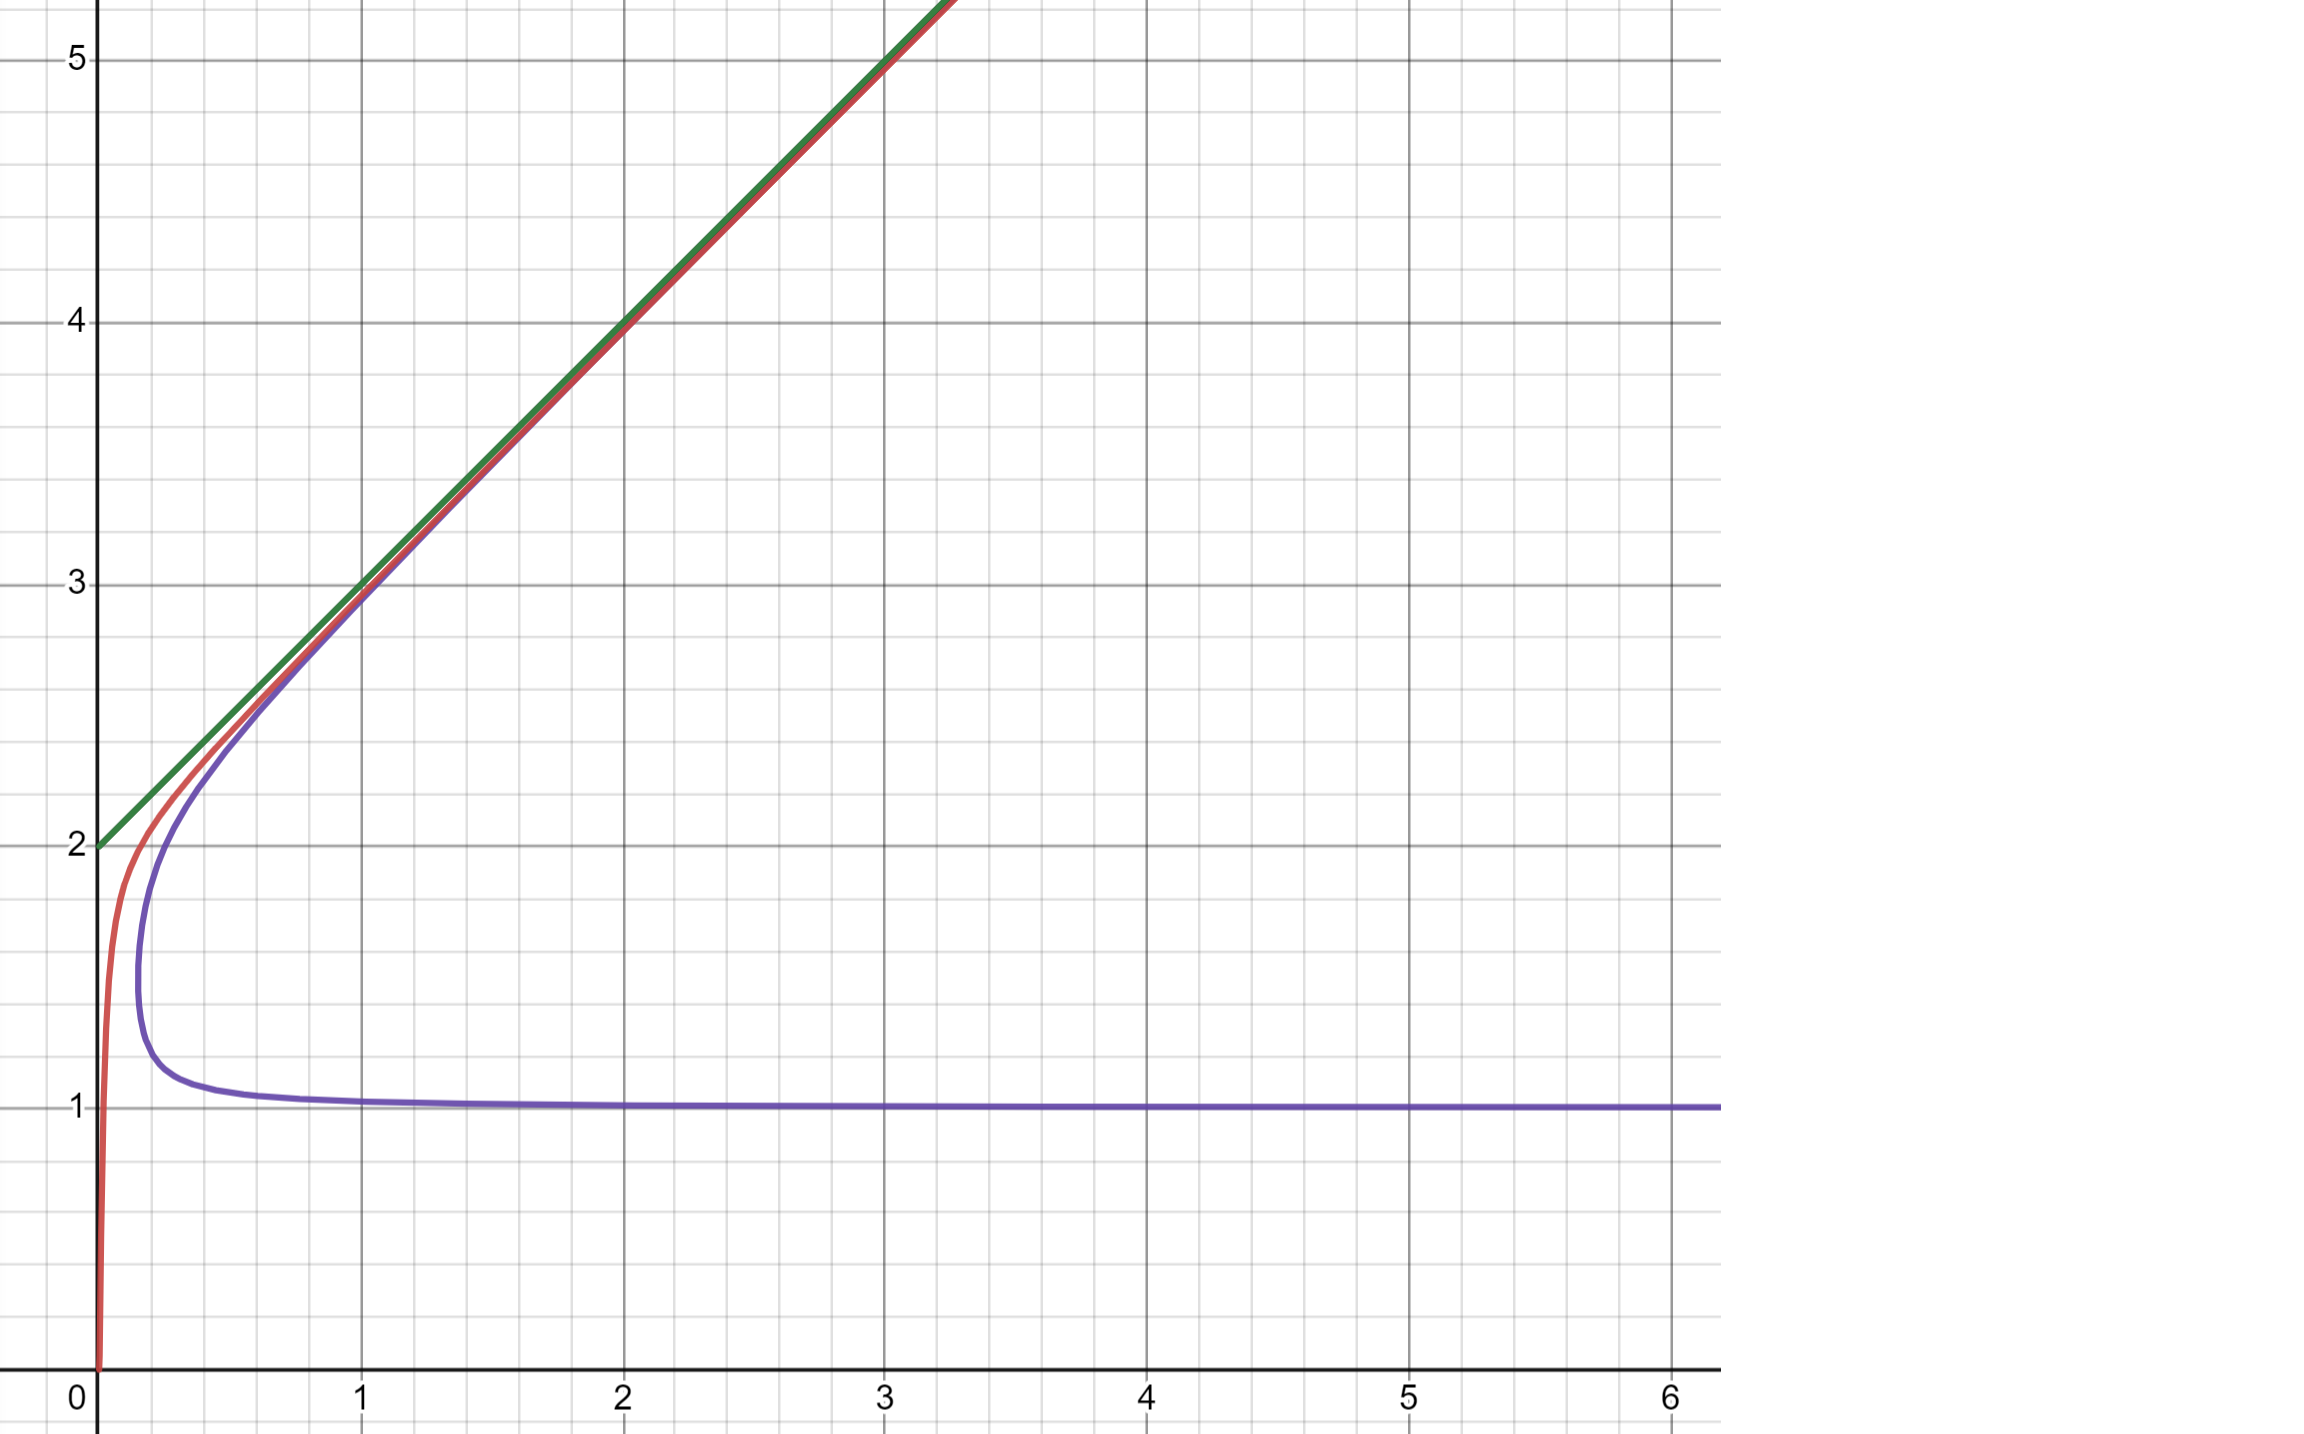
\includegraphics[width=\linewidth]{./ChickenBonds_Whitepaper_growth_price.png}

The purple line depicts the fair price (y-axis) as a solution of equation $\ref{eq:same_growth_rate}$ in function of the Pending Bucket $q_p$ (x-axis) for $q_r=1$, $q_d=2$, $S=1$, $r_r=r_p=0.1$, $r_d=0.05$ and a fixed $\alpha=30$. 

The red line shows the fair price for the controlled version for a $T_t=30$ and a variable $\alpha$.

As a reference, the naive fair price given by formula \ref{eq:naive-3} is shown in green. We can clearly see that the upper branch of the purple curve as well as the red curve approximate the naive fair price formula (equation $\ref{eq:naive-3}$) for sufficiently large $q_p$. 

This basically means that the naive fair price formula satisfies the property that the Treasury value and the bTKN supply grow at the same rate under the assumption that current users keep recycling their bonds (and no new users are creating bonds).

\pagebreak

What happens if we discount the effect of $q_p$ on the fair price by setting $c_p=0.7$ for example?

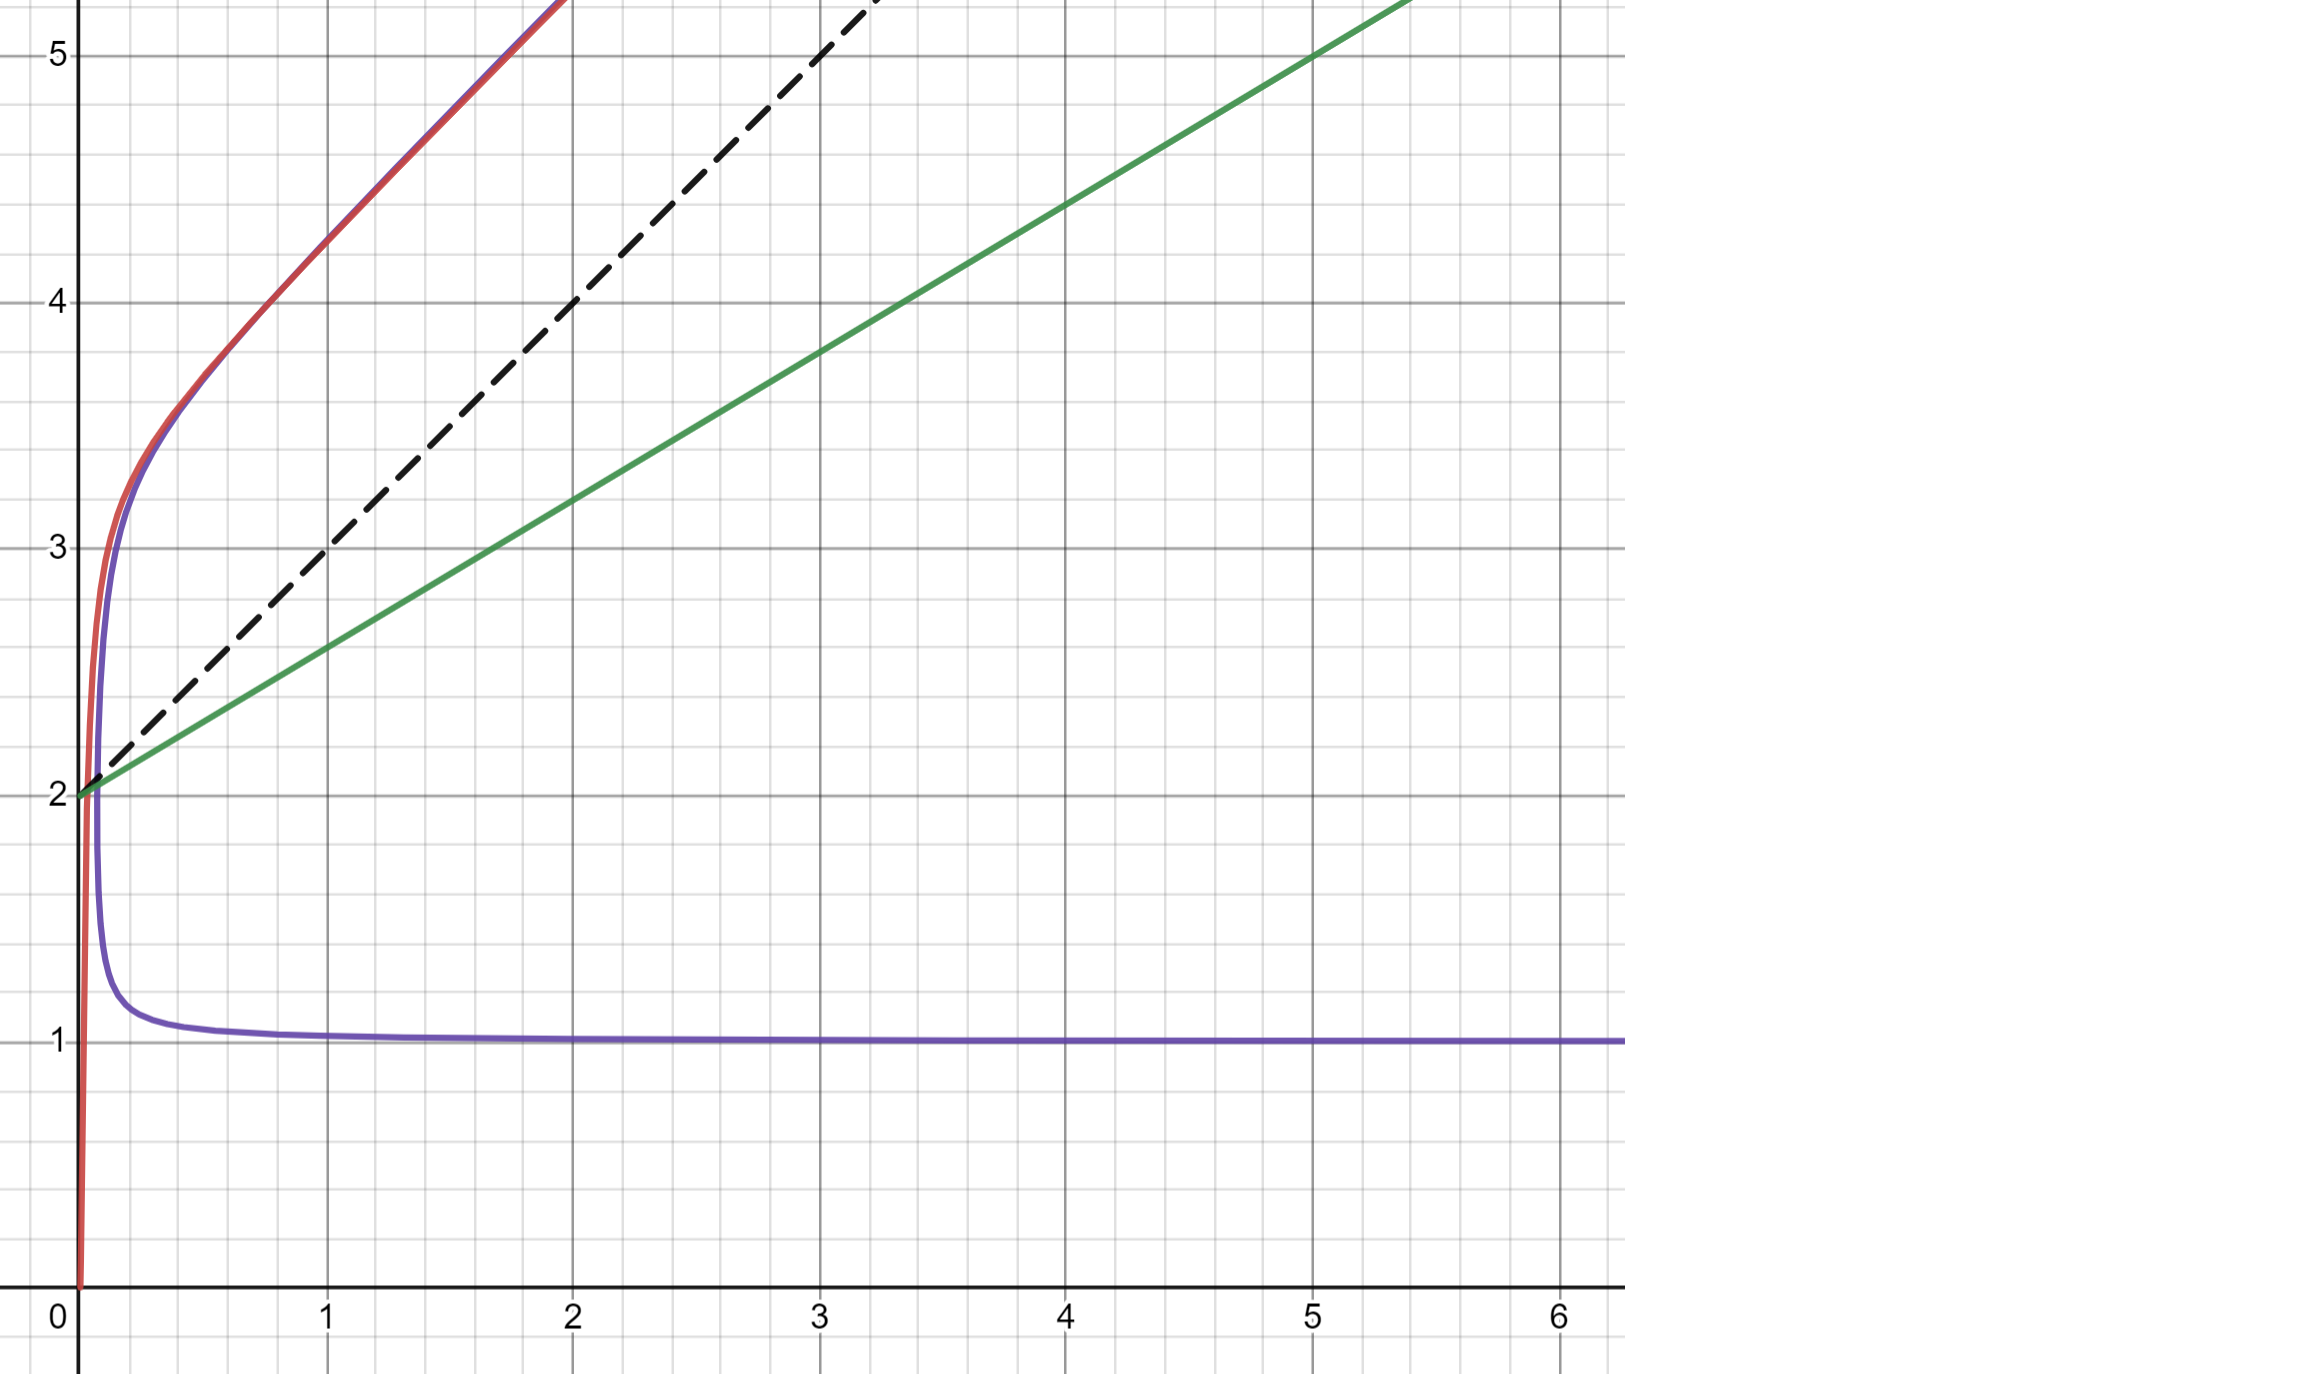
\includegraphics[width=\linewidth]{./ChickenBonds_Whitepaper_growth_price_2.png}

Note that the two versions of the fair price resulting from $\ref{eq:same_growth_rate}$ are still very similar for large $q_p$. However, they now diverge from the corrected fair price formula shown in green given by:

\begin{equation}
  \label{eq:corrected-naive}
   p_f = \frac{q_r + 0.7q_p + q_d \frac{r_d}{r_r} d_f}{S}
\end{equation}

This seems to imply that only the naive fair price formula with $c_p=1$ satisfies the property of an equal growth of $R_v$ and $S$. 

%Observation: only naive fair price formula without correction factor fulfills property for all $c_p$

%Observation: fair price does NOT make rebonding neutral with regard to the fair price if r_d =/= r_m. Price goes up if r_d>r_m. If the two rates are equal, then rebonding is neutral regardless of the chicken in time iff c_o = 1.

%Conclusion: the naive fair price formula fulfills the property, meaning that we don't need to discount the pending bucket just for the fact of being pending.

%General conclusion: too many constraints influencing $p_f$

%Regarding $q_d$, we can take the correction factor $c_d=q_d \frac{r_d}{r_r}$ from the naive formula above (equation \ref{eq:naive-3}). For $q_p$ we suppose that the Pending Bucket will eventually transition into the Reserve and the Permanent Buckets according to a split determined by the optimal rebonding time. In other words, we're discounting the fraction of the Pending Bucket with $c_p$ that we expect to become part of the Permanent Bucket, neglecting the possibility of chicken outs.

\paragraph{Immediate effect of rebonding on the fair price}
Can we thus deduct that (optimal) rebonding has no direct impact on the naive fair price at all?

It turns out that this is only true for the special case where $r_d = r_r$. Otherwise, the result may look like this:

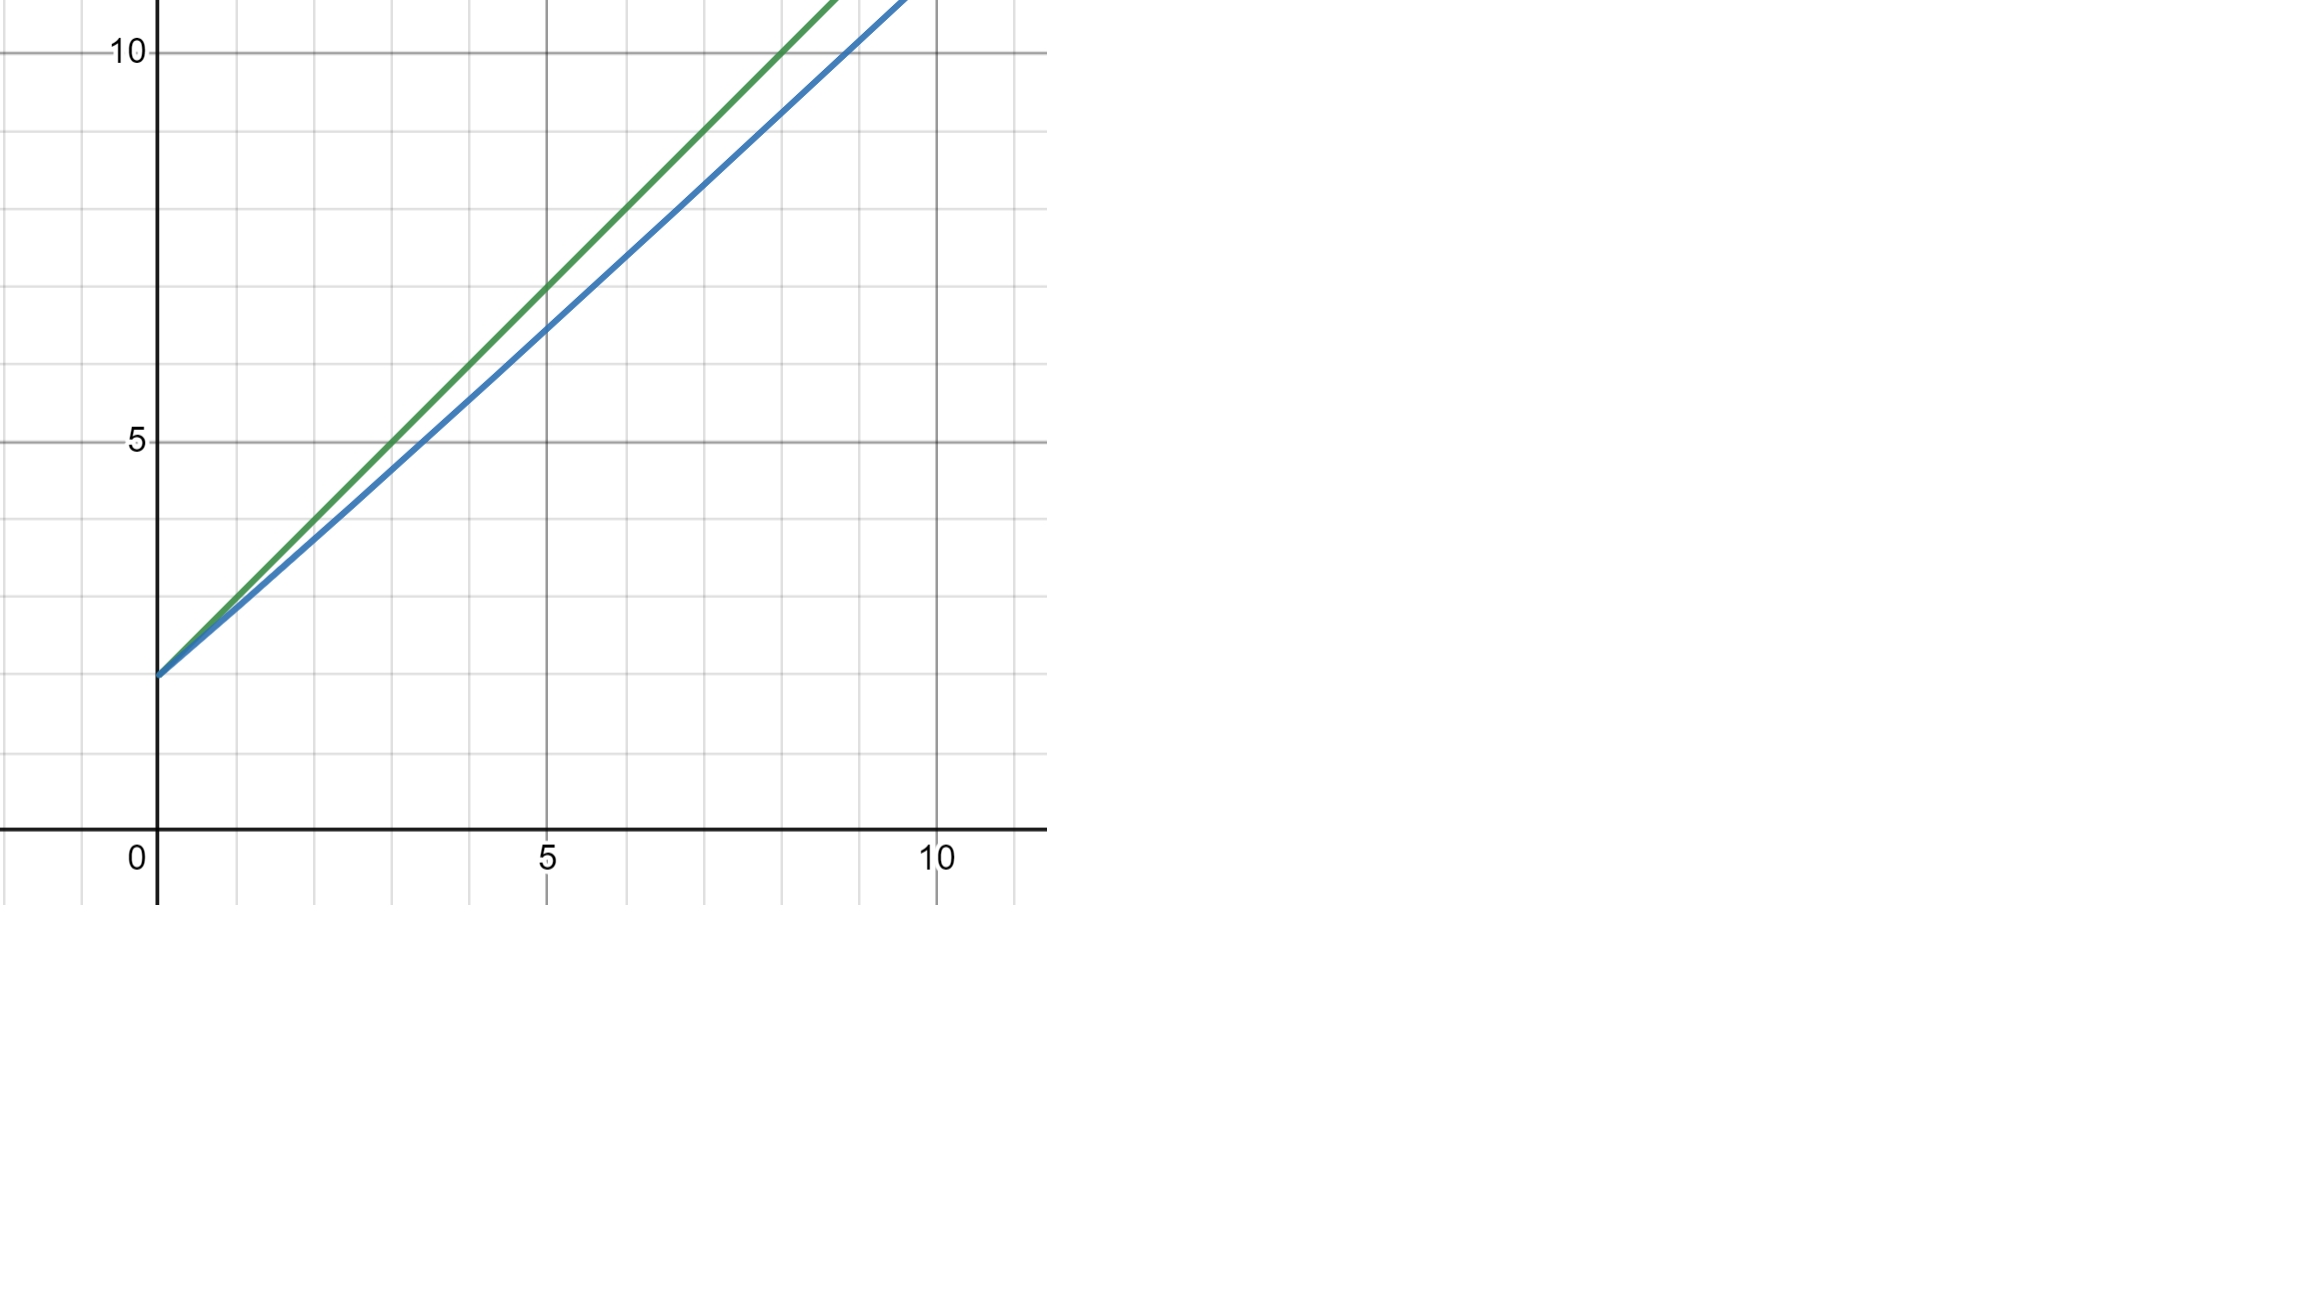
\includegraphics[width=\linewidth]{./ChickenBonds_Whitepaper_rebonding.png}

For $r_d < r_r$, rebonding negatively impacts the fair price, as can be seen in the chart above which shows the fair price before (green) and after (blue) rebonding the entire Pending Bucket at $T_{opt}$ for $q_r=1$, $q_d=2$, $S=1$, $r_r=r_p=0.1$, $r_d=0.05$ and a fixed $\alpha=30$. 

This intuitively makes sense since it results in a larger portion of $R$ earning a lower yield (the later users chicken in and rebond, the larger the effect). 

On the other hand, the parameter $\alpha$ has no influence on the resulting price curve, which also doesn't depend on whether the controller is turned on or not (and what time $T_t$ it targets).

One explanation for this seemingly contradictory result could be that while rebonding as such negatively impacts the naive fair price, the (higher) yield on the Pending Bucket compensates for this, ensuring that the Treasury and the bTKN supply grow at the same rate as a whole.

\subsubsection{Recursive approach}
Instead of assuming that the effects of chicken ins and rebonding cancel out as in the naive approach ($\ref{sec:naive_approach}$), we can try to estimate the future changes to the buckets based on historic user behavior or expected optimal behavior.

For changes to the TKN quantities inside the buckets, we use the notation $\Delta q_{r}$, $\Delta q_{p}$ and $\Delta q_{d}$ and let $P_{In}$ denote the probability that a bond holder chickens in, and $P_{Out}$ that the holder chickens out.

Assuming an infinitely fine-grained user base, we can apply these probabilities to all users in aggregate (i.e. the buckets as such), allowing us to model the overall flows between the buckets.

With that we can express the fair price $p_f$ in a recursion step as

\begin{equation}
  \label{}
    p_{f} = \frac{q_{b}+q_{p}(1-P_{In}-P_{Out})+(q_{r}+ P_{In}\Delta q_{r})+(q_{d} + P_{In}\Delta q_{d})\frac{r_{d}}{r_{m}}d_{d}}{S_{sLQTY} + \frac{P_{In}\Delta q_r}{p_r}}
\end{equation}

where $q_{b}$ stands for the amount bonded at the end of recursion step. As $p_r = \frac{q_r}{S_{sLQTY}}$, we can express the above equation as:

\begin{equation}
  \label{eq:recursive_hist}
    p_{f} = \frac{q_{b}+q_{p}(1-P_{In}-P_{Out})+(q_{r}+ P_{In}\Delta q_{r})+(q_{d} + P_{In}\Delta q_{d})\frac{r_{d}}{r_{m}}d_{d}}{S_{sLQTY} \left( 1+P_{In} \Delta q_{r} \frac{1}{q_{r}} \right)}
\end{equation}

Assumptions:

\begin{enumerate}
	\item $P_{In} + P_{Out} \leq 1$
	\item $P_{Out} = 0$, as long as bonding is profitable
	\item $P_{Out} = 1$ if bonding is not profitable
	\item There is no user churn. Current users keep rebonding.
\end{enumerate}

We further assume for simplicity that bonding activity is more or less evenly distributed over time and that bonders who got past their optimal rebonding time chicken in with $P_{In}=1$, while nobody chickens in before reaching that point.
This way, we can split the group of bonders into two segments, the ones before and the ones after the rebonding

We model $P_{In}$ by setting it to the inverse of the optimal rebonding time.

\begin{equation}
    P_{In} = \min \left(1,\frac{1}{T_{opt}}\right)
\end{equation} 

\paragraph{Bucket changes based on history}
We can estimate $\Delta q_{r}$ and $\Delta q_{d}$ based on the historic average, assuming that users would rebond when reaching the same fraction of their cap as in the past:

\begin{equation}
\Delta q_{r} = q_{p} \frac{q_{r}}{q_{r}+q_{d}}
\end{equation}

\begin{equation}
\Delta q_{d} = q_{p} \frac{q_{d}}{q_{r}+q_{d}}
\end{equation}

There should also exist an historical average rebonding period $\overline{T}$ corresponding to the current relation between $q_r$ and $q_d$:

\begin{equation}
    \frac{q_{r}}{q_{r}+q_{d}} = \frac{\overline{T}}{\overline{T}+1}
\end{equation}

\begin{equation}
    \overline{T} = \frac{q_{r}}{q_{d}}
\end{equation}

Even though $\overline{T}$ may not necessarily reflect the optimal rebonding strategy, we can use it to estimate $P_{In}$:

\begin{equation}
   P_{In} = \frac{1}{\overline{T}} = \frac{q_{d}}{q_{r}}
\end{equation}

This leads to the following fair price (where $q_b$ stands for the rebonded amount):

\[
p_{f} = \frac{q_{b}+q_{p} \left(1-\frac{q_{d}}{q_{r}}\right)+\left(q_{r}+\frac{q_{d}}{q_{r}}q_{p}\frac{q_{r}}{q_{r}+q_{d}}\right)+ \left(q_{d}+\frac{q_{d}}{q_{r}}q_{p}\frac{q_{d}}{q_{r}+q_{d}}\right)\frac{r_{d}}{r_{m}}d_{d}}{S_{sLQTY} \left( 1+\frac{q_{d}}{q_{r}} q_{p}\frac{q_{r}}{q_{r}+q_{d}}\frac{1}{q_{r}} \right)}
\]

\[
p_{f} = \frac{q_{b}+q_{p} \left(1-\frac{q_{d}}{q_{r}}\right)+q_{r}\left(1+\frac{q_{d}}{q_{r}}\frac{q_{p}}{q_{r}+q_{d}}\right)+q_{d} \left(1+\frac{q_{d}}{q_{r}}\frac{q_{p}}{q_{r}+q_{d}}\right)\frac{r_{d}}{r_{m}}d_{d}}{S_{sLQTY} \left( 1+\frac{q_{d}}{q_{r}}\frac{q_{p}}{q_{r}+q_{d}} \right)}
\]

\begin{equation}
p_{f} = \frac{q_{b}+q_{p} \left(1-\frac{q_{d}}{q_{r}}\right)}{S_{sLQTY} \left( 1+\frac{q_{d}}{q_{r}}\frac{q_{p}}{q_{r}+q_{d}} \right)} + \frac{q_{r}+q_{d}\frac{r_{d}}{r_{m}}d_{d}}{S_{sLQTY}}
\end{equation}

Assuming all rebonders can sell their bTKN at the fair price without incurring any slippage, we can express $q_b$ as follows:

\begin{equation}
q_{b} = p_f P_{In} \Delta q_{r} \frac{1}{p_r} = \frac{q_{d}}{q_{r}} q_p \frac{q_{r}}{q_{r}+q_{d}} \frac{p_{f}}{p_{r}}  = q_p \frac{q_{d}}{q_{r}+q_{d}} \frac{p_{f}}{p_{r}}
\end{equation}

Resulting in:

\begin{equation}
p_{f} = \frac{q_{p} \left(1+\frac{q_{d}}{q_{r}+q_{d}} \frac{p_{f}}{p_{r}}-\frac{q_{d}}{q_{r}}\right)}{S_{sLQTY} \left( 1+\frac{q_{d}}{q_{r}}\frac{q_{p}}{q_{r}+q_{d}} \right)} + \frac{q_{r}+q_{d}\frac{r_{d}}{r_{m}}d_{d}}{S_{sLQTY}}
\end{equation}

\paragraph{Bucket changes based on optimal rebonding strategy}
One could use the optimal (future) rebonding time instead of deducting the historical average:

\begin{equation}
\Delta q_{r} = q_{p} \frac{T_{opt}}{T_{opt}+1}
\end{equation}

\begin{equation}
\Delta q_{d} = q_{p} \left( 1- \frac{T_{opt}}{T_{opt}+1} \right)
\end{equation}

This leads to:

\[
p_{f} = \frac{q_{b}+q_{p} \left(1-\frac{1}{T_{opt}}\right)+\left(q_{r}+\frac{1}{T_{opt}} q_{p} \frac{T_{opt}}{T_{opt}+1}\right)+ \left(q_{d}+\frac{1}{T_{opt}} q_{p} \left( 1- \frac{T_{opt}}{T_{opt}+1}\right)\right)\frac{r_{d}}{r_{m}}d_{d}}{S_{sLQTY} \left( 1+\frac{1}{T_{opt}} q_{p} \frac{T_{opt}}{T_{opt}+1}\frac{1}{q_{r}} \right)}
\]

\[
p_{f} = \frac{q_{b}+q_{p} \left(1-\frac{1}{T_{opt}}\right)+\left(q_{r}+ \frac{q_{p}}{T_{opt}+1}\right)+ \left(q_{d}+\frac{q_{p}}{T_{opt}} - \frac{q_{p}}{T_{opt}+1}\right)\frac{r_{d}}{r_{m}}d_{d}}{S_{sLQTY} \left( 1+ \frac{1}{T_{opt}+1}\frac{q_{p}}{q_{r}} \right)}
\]

\[
p_{f} = \frac{q_{b}+q_{p}\left(1-\frac{1}{T_{opt}}\right)+q_{r}+ \frac{q_{p}}{T_{opt}+1}+\left(q_{d}+q_{p} \left( \frac{1}{T_{opt}}- \frac{1}{T_{opt}+1} \right)\right)\frac{r_{d}}{r_{m}}d_{d}}{S_{sLQTY}\left(1+  \frac{1}{T_{opt}+1}\frac{q_{p}}{q_{r}}\right)}
\]

\begin{equation}
  \label{eq:recursive_optimal_1}
p_{f} = \frac{q_{b}+q_{p} \left(1+\frac{1}{T_{opt}}\left(\frac{r_{d}}{r_{m}}d_{d}-1\right)+ \frac{1}{T_{opt}+1}\left( 1 - \frac{r_{d}}{r_{m}}d_{d} \right)\right)+q_{r}+q_{d}\frac{r_{d}}{r_{m}}d_{d}}{S_{sLQTY}\left(1+  \frac{1}{T_{opt}+1}\frac{q_{p}}{q_{r}}\right)}
\end{equation}

With $\frac{r_{d}}{r_{m}}d_{d}=1$

\begin{equation}
  \label{eq:recursive_optimal_2}
p_{f} = \frac{q_{b}+q_{p}+q_{r}+q_{d}}{S_{sLQTY}\left(1+  \frac{1}{T_{opt}+1}\frac{q_{p}}{q_{r}}\right)}
\end{equation}

For constant rebonding:

\begin{equation}
q_{b} = q_{p} \frac{1}{T_{opt}} \frac{T_{opt}}{T_{opt}+1}\frac{p_{f}}{p_{r}} = \frac{q_{p}}{T_{opt}+1}\frac{p_{f}}{p_{r}}
\end{equation}

This leads to:

\[
p_{f} = \frac{ \frac{q_{p}}{T_{opt}+1}\frac{p_{f}}{p_{r}}+q_{p} \left(1+\frac{1}{T_{opt}}\left(\frac{r_{d}}{r_{m}}d_{d}-1\right)+ \frac{1}{T_{opt}+1}\left( 1 - \frac{r_{d}}{r_{m}}d_{d} \right)\right)+q_{r}+q_{d}\frac{r_{d}}{r_{m}}d_{d}}{S_{sLQTY}\left(1+  \frac{1}{T_{opt}+1}\frac{q_{p}}{q_{r}}\right)}
\]

\begin{equation}
p_{f} = \frac{q_{p} \left(1 + \frac{1}{T_{opt}}\left(\frac{r_{d}}{r_{m}}d_{d}-1\right)+ \frac{1}{T_{opt}+1}\left(\frac{p_{f}}{p_{r}} + 1 - \frac{r_{d}}{r_{m}}d_{d} \right)\right)+q_{r}+q_{d}\frac{r_{d}}{r_{m}}d_{d}}{S_{sLQTY}\left(1+  \frac{1}{T_{opt}+1}\frac{q_{p}}{q_{r}}\right)}
\end{equation}

With $\frac{r_{d}}{r_{m}}d_{d}=1$

\begin{equation}
p_{f} = \frac{q_{p} \left( 1+   \frac{1}{T_{opt}+1}\frac{p_{f}}{p_{r}} \right)+q_{r}+q_{d}}{S_{sLQTY}\left(1+  \frac{1}{T_{opt}+1}\frac{q_{p}}{q_{r}}\right)}
\end{equation}

We have tried to validate results from this section without success. For instance below we have charts for the historic variant of the recursive approach. We can see non-convergence and really weird behaviour starting from iteration 10:

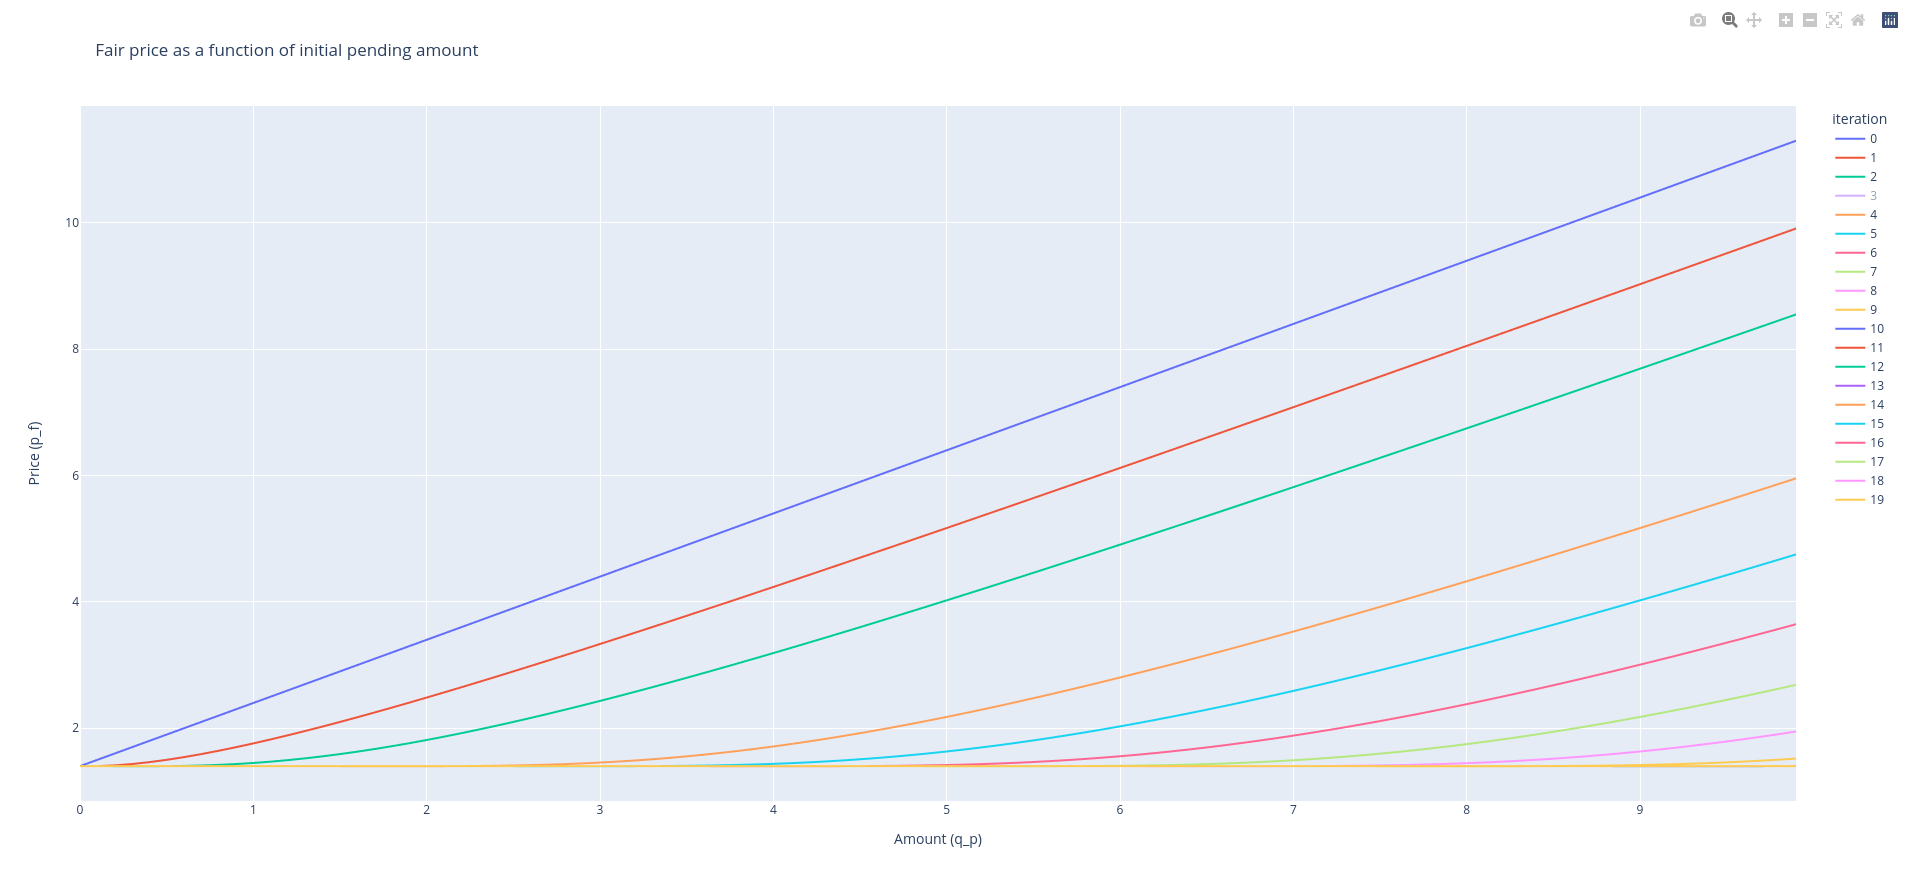
\includegraphics[width=\linewidth]{./ChickenBonds_Whitepaper_recursive_price_1.png}

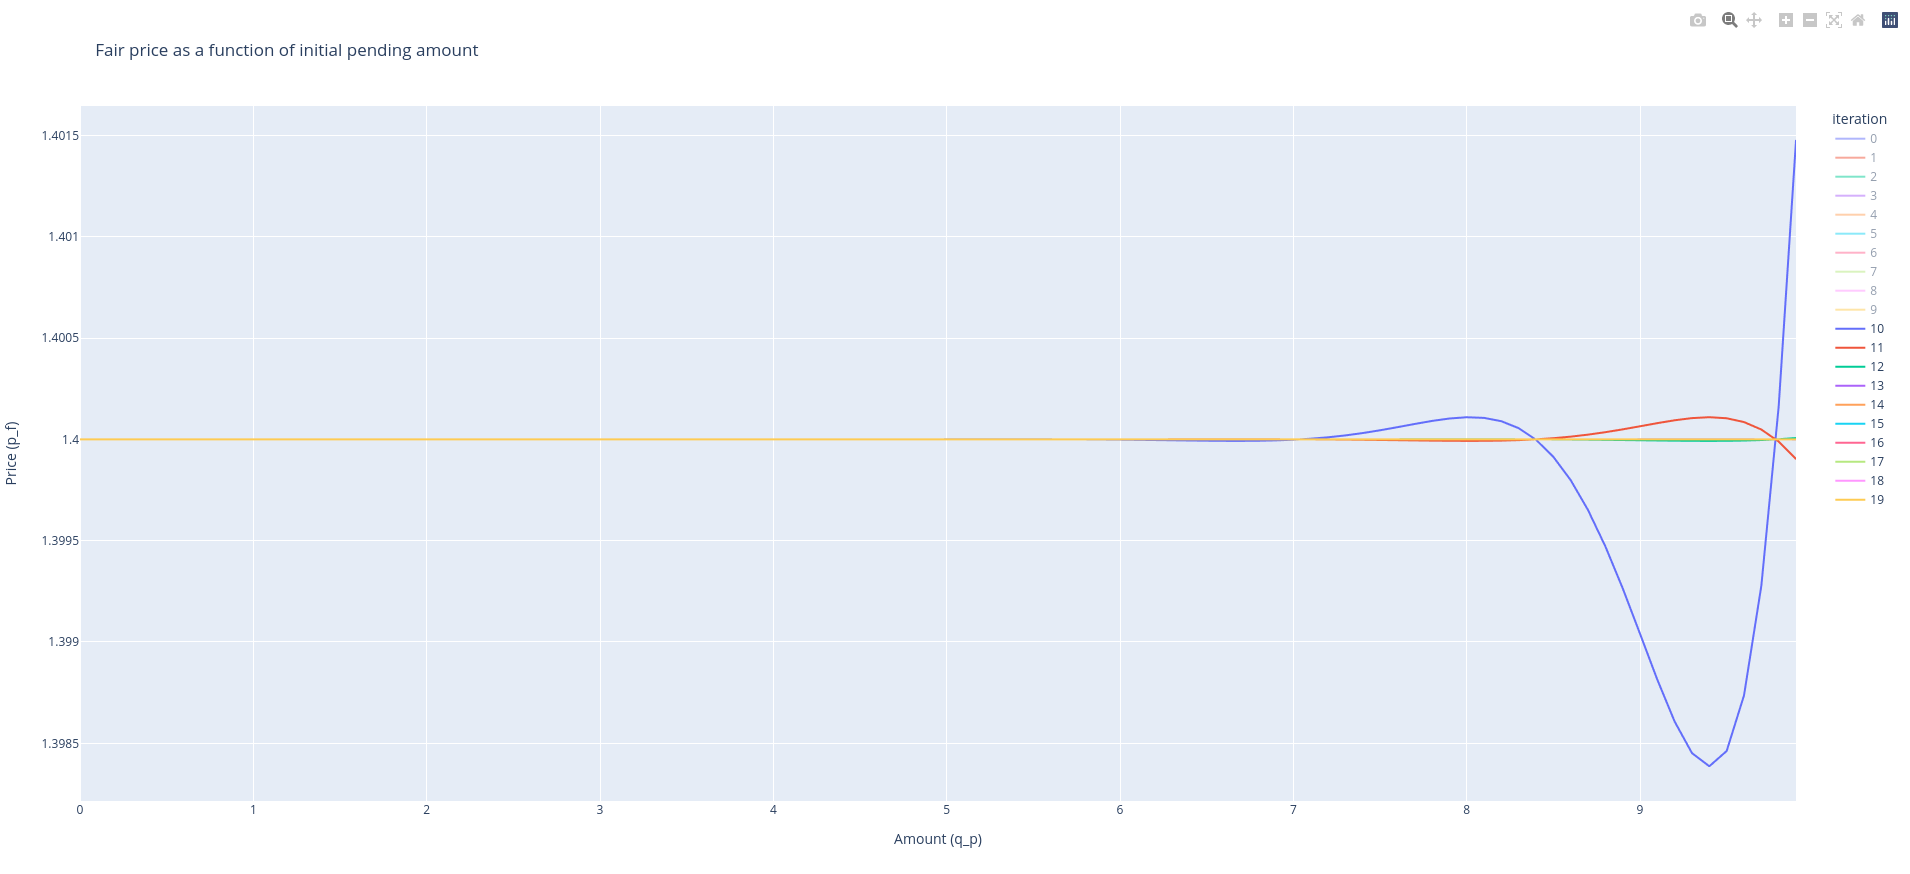
\includegraphics[width=\linewidth]{./ChickenBonds_Whitepaper_recursive_price_2.png}

\subsubsection{Yield comparison approach}
We can also consider the evolution of the fair price of bTKN over a given time period and compare it with an expected yield. In the following, we outline two different approaches.

\paragraph{Equating ROI of bonding TKN and holding bTKN}
We suppose that users would bond TKN rather than hold bTKN if the expected ROI from bonding is higher than of (buying and) holding bTKN, and vice versa. As long as holding bTKN is more attractive than bonding TKN, we can expect buying pressure on bTKN. Conversely, there should be selling pressure on bTKN if bonding is seen as more profitable since people would likely trade their bTKN for TKN. 

As a consequence, there must be an equilibrium price at which holding bTKN and bonding TKN result in the same ROI for both activities. Due to the yield amplification, it's safe to assume that in the long run, holding bTKN is at least as profitable as the underlying yield producing strategy for TKN. We further assume that the price of TKN is already “arbitraged” and adapted to the natural rate $r_m$, which thus carries over to the price of bTKN. Therefore, the equilibrium price for bonding vs. holding should also be meaningful as a metric for the fair price.

\subparagraph{With constant $\alpha$}
We consider one optimal rebonding period $T_{opt}$ with a fixed parameter $\alpha$ and suppose that the system is "frozen" during that time frame, i.e. nobody chickens in or out and no new bonds are created. Since the protocol is still earning yield on its treasury $R$, the only quantity that would change during the respective period is $q_r$, but we can neglect the compounding effect for small $r_r$, $r_p$ and $r_d$ and short $T_{opt}$, treating $R$ as constant.

Further, we make the simplifying assumption that the price premium $\lambda$ stays constant during that time frame. Thus, the fair price $p_f$ changes from $t$ to $t+T_{opt}$ at the same rate as the redemption price $p_r$, yielding the ROI of holding bTKN:

\begin{equation}
  \label{eq:ROI-eq}
  H_{ROI} = \frac{p_f(t + T_{opt}) - p_f(t)}{p_f(t)} = \frac{p_r(t + T_{opt}) - p_r(t)}{p_r(t)}
\end{equation}

The resulting redemption price at time $t + T_{opt}$ can be expressed by
\begin{equation}
  \label{eq:redemption-price}
    p_r(t + T_{opt}) = \frac{q_r + \frac{T_{opt}}{365} (r_p q_p + r_r q_r + r_d q_d)}{S}
\end{equation}

yielding:
\begin{equation}
  \label{eq:ROI-eq2}
  \begin{split}
    H_{ROI} & = \frac{\frac{q_r + \frac{T_{opt}}{365} (r_p q_p + r_r q_r + r_d q_d)}{S} - p_r(t)}{p_r(t)} \\
    & = \frac{q_r}{S \cdot p_r(t)} + \frac{\frac{T_{opt}}{365} (r_p q_p + r_r q_r + r_d q_d)}{S\cdot p_r(t)} - \frac{p_r(t)}{p_r(t)} \\
    & = 1 + \frac{T_{opt}}{365} \frac{r_p q_p + r_r q_r + r_d q_d}{q_r} - 1 \\
    & = \frac{T_{opt}}{365} \frac{r_p q_p + r_r q_r + r_d q_d}{q_r}
  \end{split}
\end{equation}

On the other hand, we can express the ROI of bonding TKN for the same period as:

\begin{equation}
  \label{eq:ROI-bonding}
  \begin{split}
    B_{ROI} & = \frac{p_f(t+T_{opt})}{p_r(t+T_{opt})}\frac{T_{opt}}{T_{opt}+\alpha} - 1 \\
    & = \frac{p_f(t)(1 + \frac{T_{opt}}{365} (r_p q_p + r_r q_r + r_d q_d))} {p_r(t)(1 + \frac{T_{opt}}{365} (r_p q_p + r_r q_r + r_d q_d))}    \frac{T_{opt}}{T_{opt}+\alpha} - 1 \\ 
    & = \frac{p_f(t)}{p_r(t)}\frac{T_{opt}}{T_{opt}+\alpha} - 1
  \end{split}
\end{equation}

Setting the two ROIs equal, we can solve the following equation for $p_f$:
\begin{equation}
  \label{eq:ROI-bonding-holding}
  B_{ROI} = H_{ROI}
\end{equation}

and get:
\begin{equation}
  \label{eq:ROI-bonding-holding-2}
  p_f = p_r\left(1 + \frac{T_{opt}}{365} \frac{r_p q_p + r_r q_r + r_d q_d}{q_r}\right) \frac{T_{opt}+\alpha}{T_{opt}}
\end{equation}

Note that, from \ref{eq:opt-rebonding-prices}, $T_{opt}$ depends on $p_f$, so we would need some more steps to isolate fair price. We can use equation \ref{eq:optimal_chicken_in_2} as an approximation of $T_{opt}$ to make it easier and get rid of the Lambert W function.

The following chart plots $p_f$ on the y-axis in function of the Pending Bucket $q_p$ (x-axis) for $\alpha$=(50, 100, 150, 200), with $q_r=1$, $q_d=2$, $S=$1 and $r_r=r_p=r_d=0.1$. As a reference, the naive fair price given by formula \ref{eq:naive-3} is shown in black.

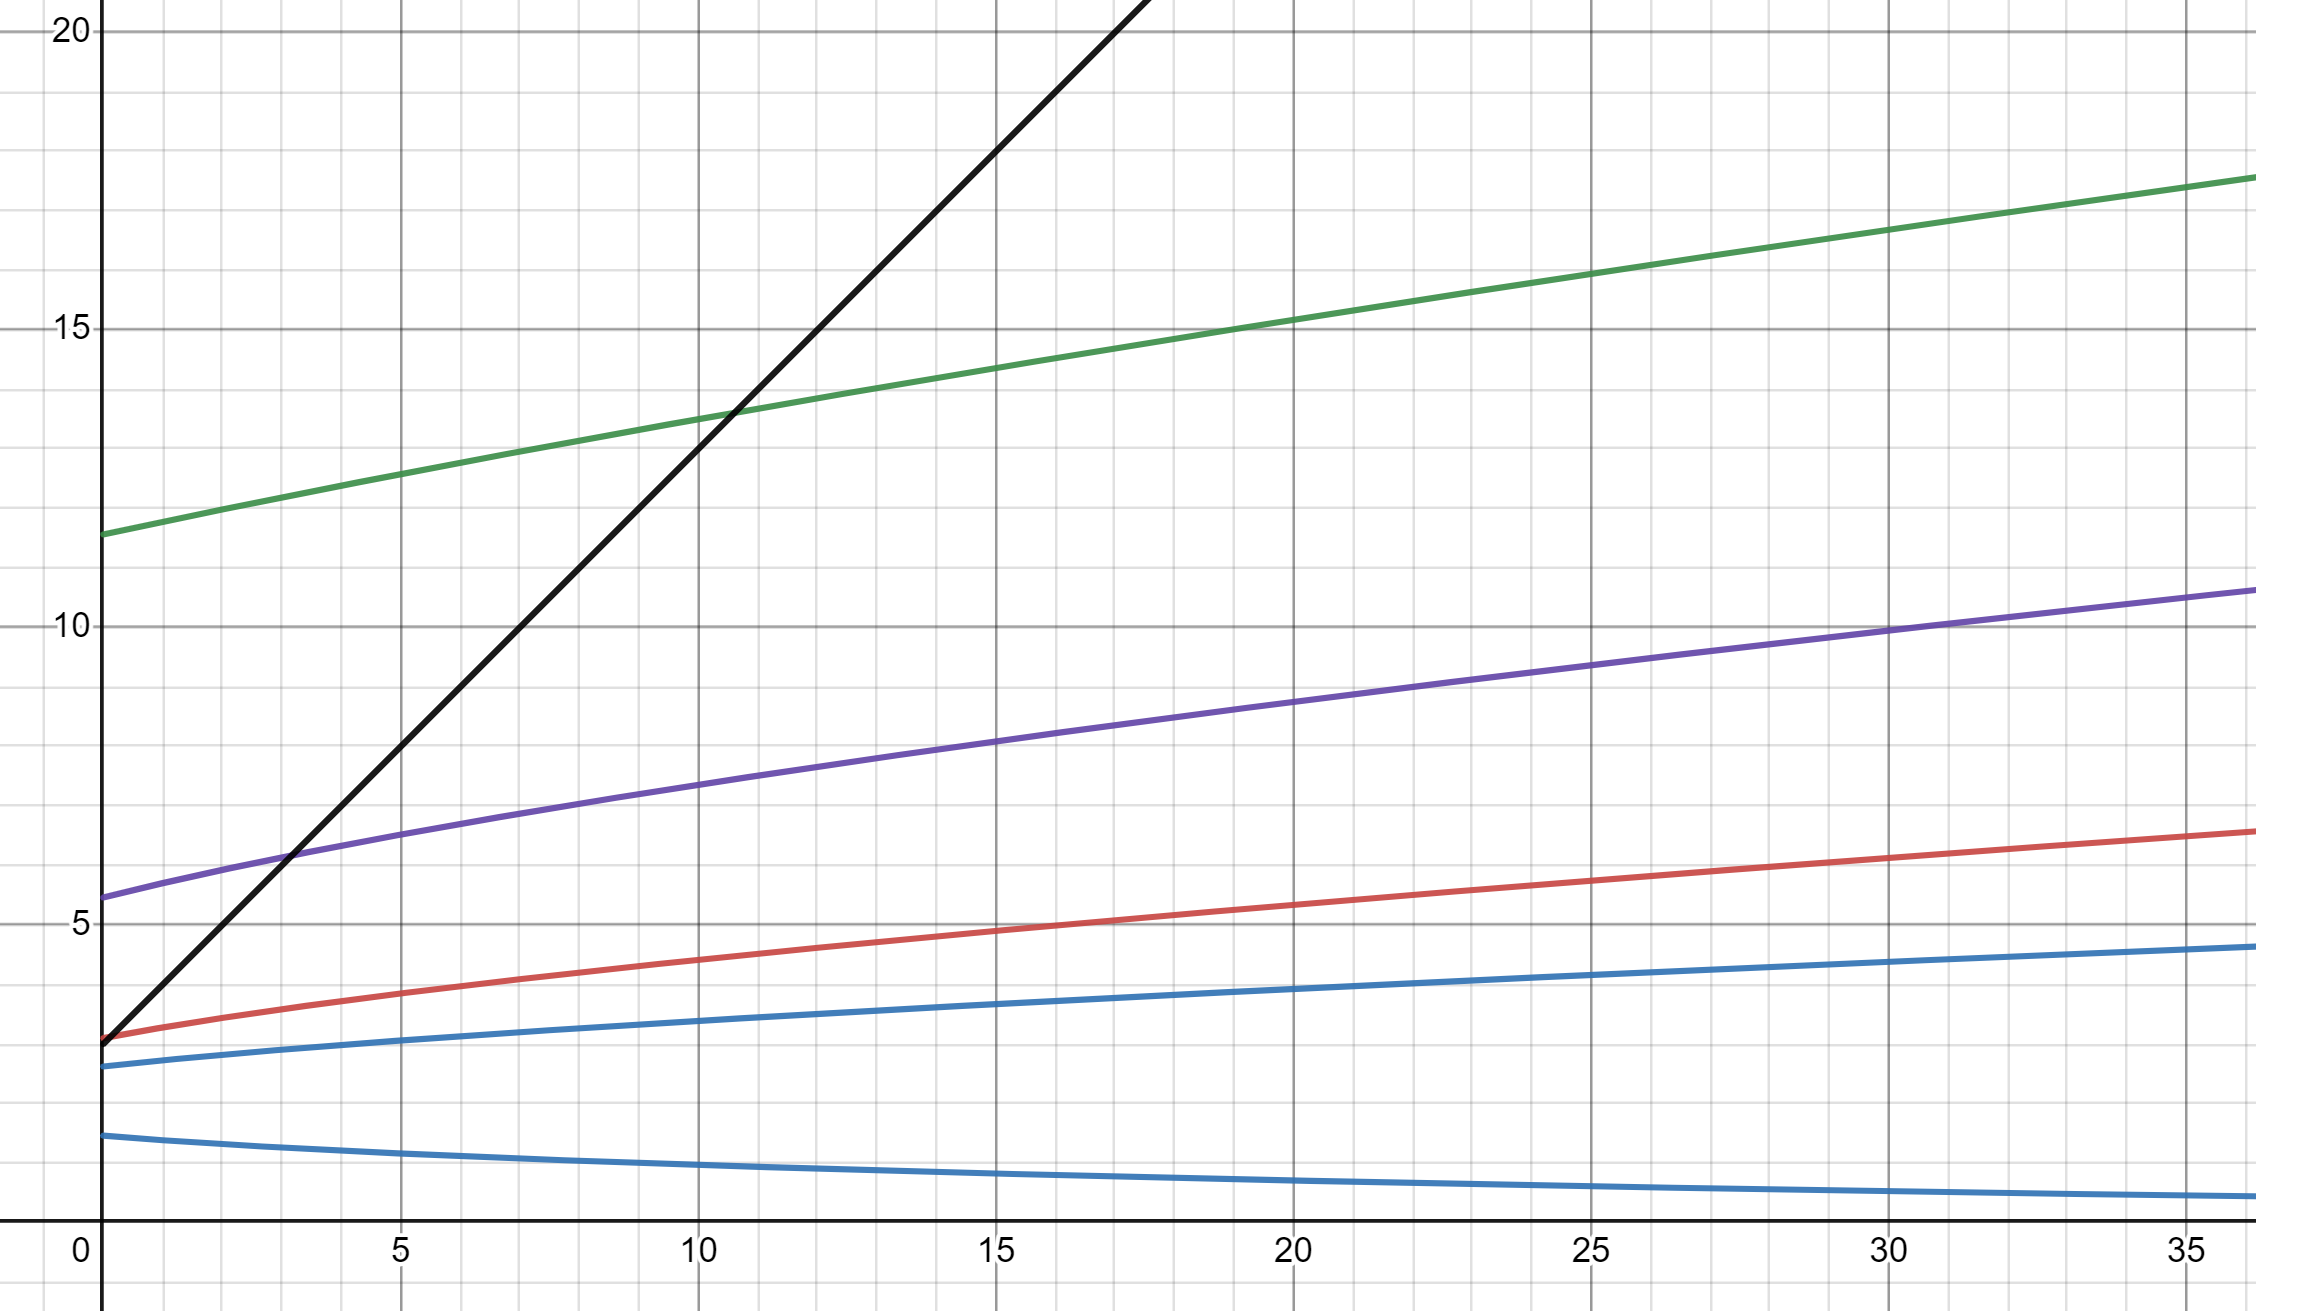
\includegraphics[width=\linewidth]{./ChickenBonds_Whitepaper_comparison_price.png}

Note that the curves are increasing for higher $\alpha$ and that all the equations have lower branches, only one of which is shown on the chart (in blue for $\alpha$=50). 

\subparagraph{With $\alpha$ being adjusted by the controller}
By assuming that the controller will keep the actual rebonding time constant (section \ref{sec:adjustment}), we can solve the approximation formula for $T_{opt}$ (equation \ref{eq:optimal_chicken_in_2}) for $\alpha$, obtaining

\begin{equation}
  \label{eq:alpha-solved}
  \alpha = T_{opt}\frac{\frac{p_f}{p_r} - 1}{1 + \sqrt{\frac{p_f}{p_r}}} = T_{opt}\frac{\lambda - 1}{1 + \sqrt{\lambda}}
\end{equation} 

In the formula for $B_{ROI}$ as defined above (equation \ref{eq:ROI-bonding}), we can substitute $\alpha$ by equation $\ref{eq:alpha-solved}$ and, after rearranging and simplifying, we get

\begin{equation}
  \label{eq:BROI-controller}
    B_{ROI} = \sqrt{\frac{p_f}{p_r}} - 1 = \sqrt{\lambda} - 1
\end{equation} 

Supposing that users will chicken in at the optimal rebonding time and given a target chicken in time $T_t$ aimed for by the controller (see section \ref{sec:adjustment}), we can replace $T_{opt}$ by $T_t$ in formula \ref{eq:ROI-eq2}:

\begin{equation}
  \label{eq:HROI-controller}
    H_{ROI} = \frac{T_t}{365} \frac{r_p q_p + r_r q_r + r_d q_d}{q_r}
\end{equation} 

Using the new definitions of $H_{ROI}$ and $B_{ROI}$, we can solve equation \ref{eq:ROI-bonding-holding} for $p_f$, obtaining

\begin{equation}
  \label{eq:ROI-bonding-holding-controller}
  p_f = p_r\left(1 + \frac{T_t}{365} \frac{r_p q_p + r_r q_r + r_d q_d}{q_r}\right)^2 
\end{equation}

The following chart depicts the fair price (y-axis) according to equation \ref{eq:ROI-bonding-holding-controller} in function of the Pending Bucket $q_p$ (x-axis) for $T_t=(60, 120, 240, 480, 960)$, with $q_r=1$, $q_d=2$, $S=1$ and $r_r=r_p=r_d=0.1$.
As a reference, the naive fair price given by formula \ref{eq:naive-3} is shown in black.

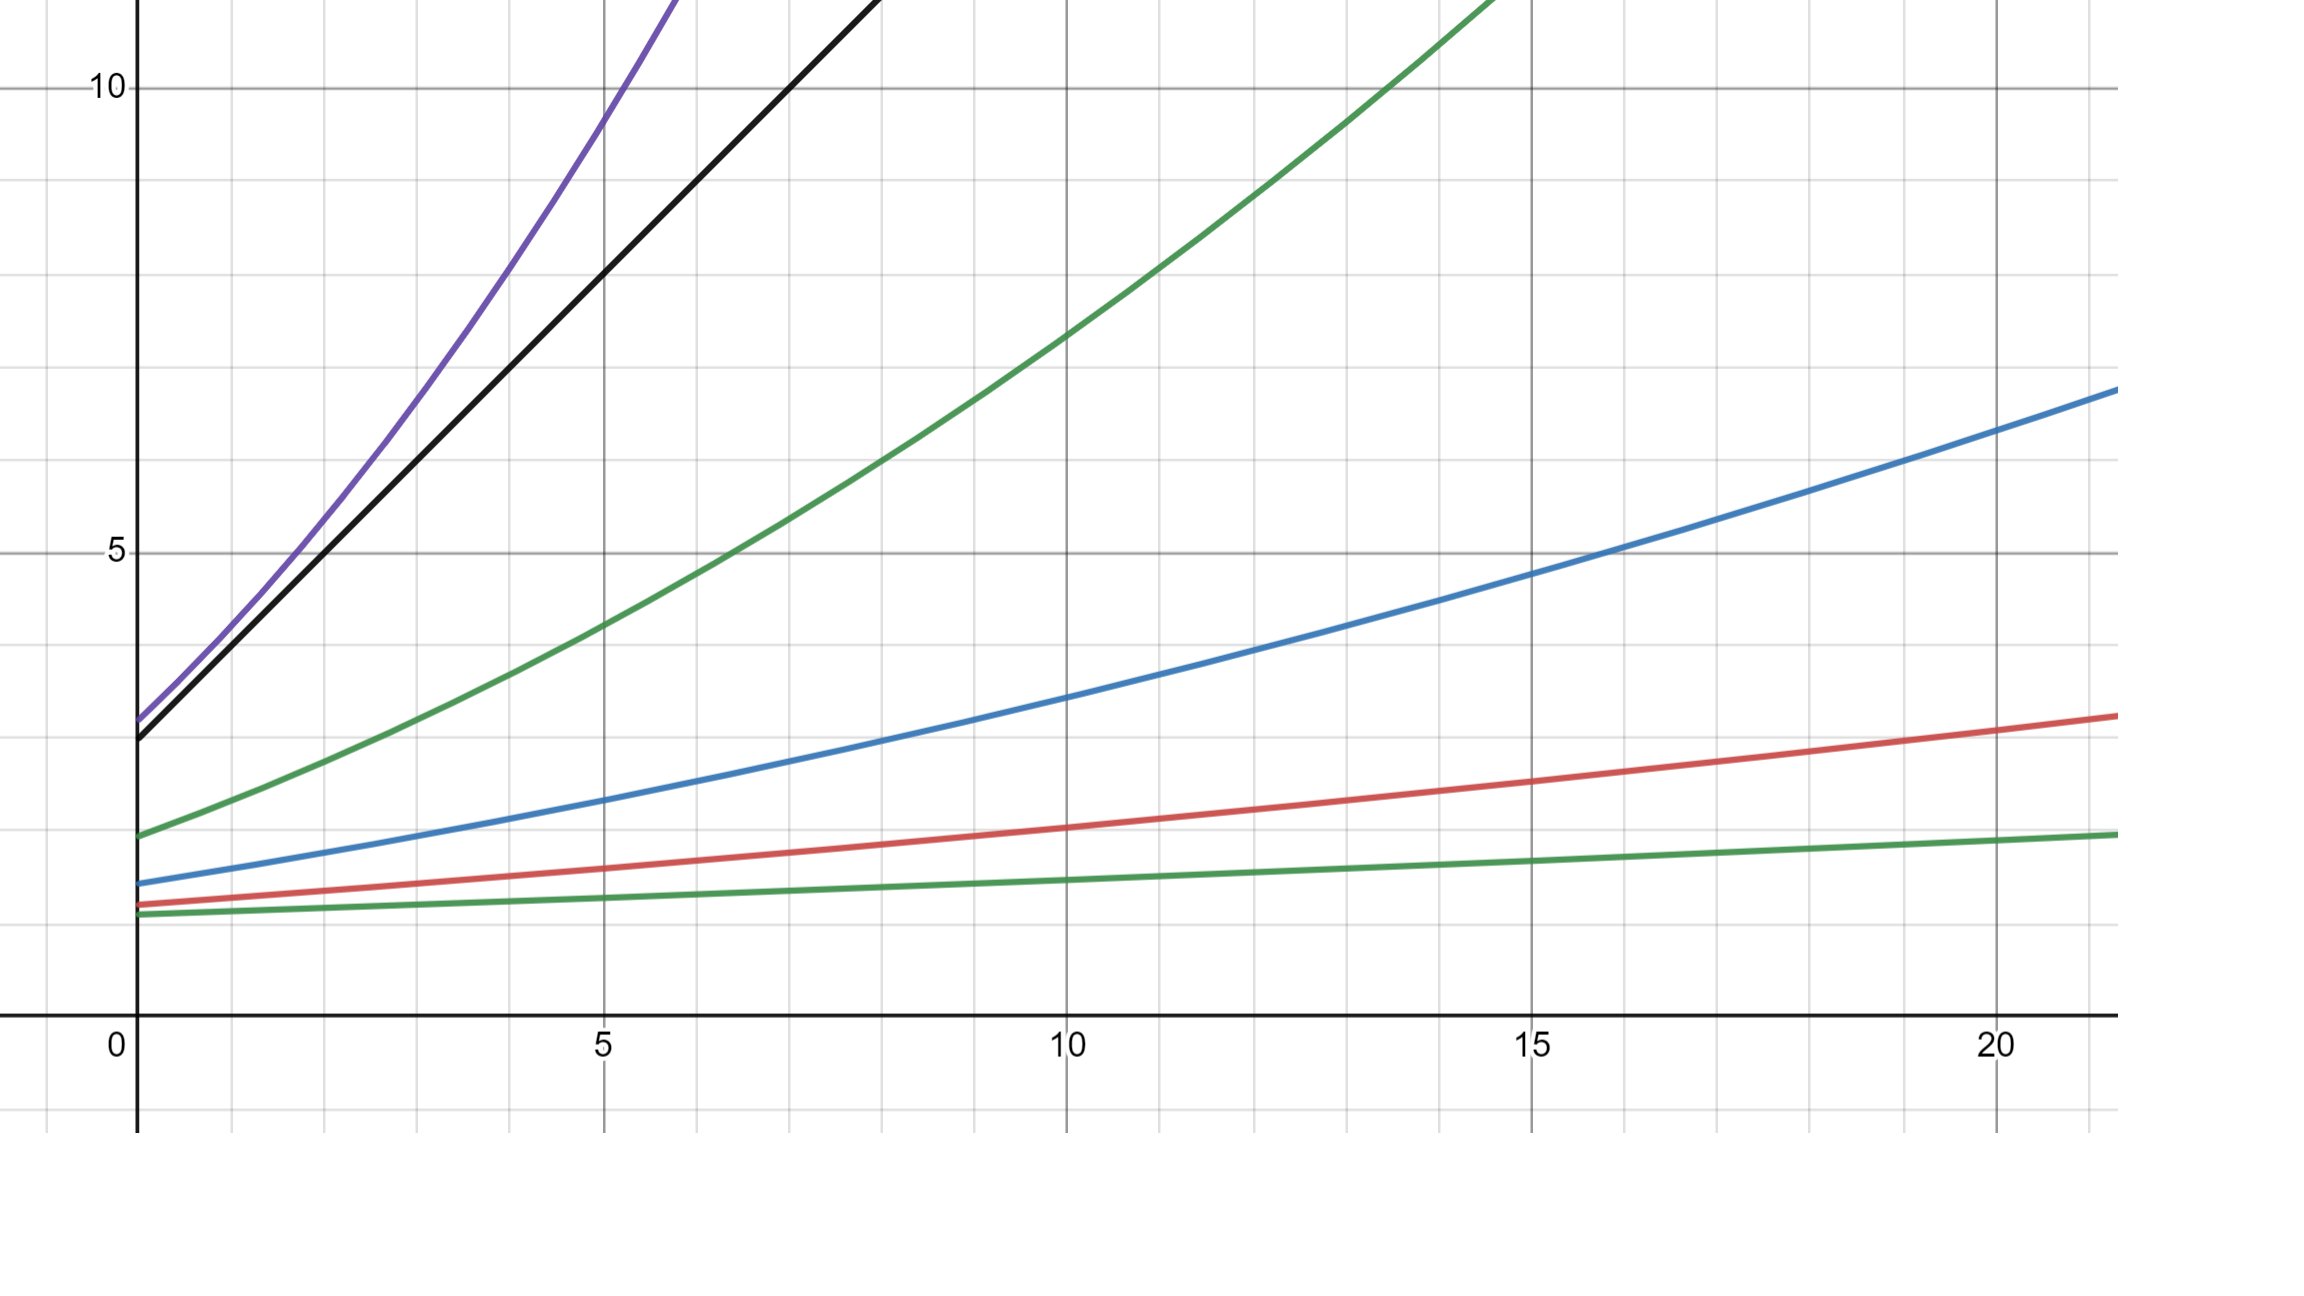
\includegraphics[width=\linewidth]{./ChickenBonds_Whitepaper_controller_price.png}

Note that the impact of $q_p$ on the fair price gets bigger for larger $T_t$, and the same is true for $q_d$ and $q_r$, which influence $p_f$ in the same fashion.

\paragraph{Equating ROI of staking TKN and holding bTKN}
Assuming rational markets and no additional risks for holding bTKN compared to holding and staking TKN (or getting yield from the underlying strategy for TKN), we suppose that the market price of bTKN would grow at the same rate as the value of staked TKN. The rationale being that if the market expects bTKN to grow faster in the future, it should pay a higher price for bTKN now, meaning that the initial price premium should reflect the future growth potential and cancel out any oversized yield from the start.

If we know what yield to expect, we could formulate a differential equation to derive a formula for $p_f$ or at least a parameter $\gamma$ for the impact of the pending bucket in the naive formula:

\begin{equation}
  \label{eq:naive-beta}
   p_f = \frac{q_r + \gamma q_p + q_d \cdot \frac{r_d}{r_r} \cdot d_f}{S}
\end{equation}

We could then state the following equation (where $r_s$ is the yield of staking TKN):

\begin{equation}
  \label{eq:yield-eq}
  \frac{p_f(t + 365) - p_f(t)}{p_f(t)} = r_s = r_m 
\end{equation}

Given that people would rebond during the course of the year, it’s simpler to consider a time period that corresponds to an optimal rebonding period for the current premium, which we suppose to be constant as long as no rebonding happens (all else being equal). This means, we assume away any new bonds and chicken-outs, and only consider the group of existing bonders which all rebond perfectly.

This allows us to reformulate the equation, which could be solved for $\gamma$:

\begin{equation}
  \label{eq:yield-eq}
  \frac{p_f(t + T_{opt}) - p_f(t)}{p_f(t)} = \frac{T_{opt}}{365} r_m
\end{equation}

\subsubsection{Conservative approach}
This approach is probably not the most accurate or realistic, but at least it can serve as a lower bound for the fair price.

Let’s imagine a user who wants to buy bTKN to sell it after some time $T$ for a profit, and, being conservative, they don’t want to rely on the bTKN valuations of other users - they simply want to make sure that redeeming their bTKN would at least result in net gains which correspond to the natural rate of TKN.

In the following chart, the red line corresponds to the natural rate, the green line to the redemption price and the purple line to the (conservative) fair price.

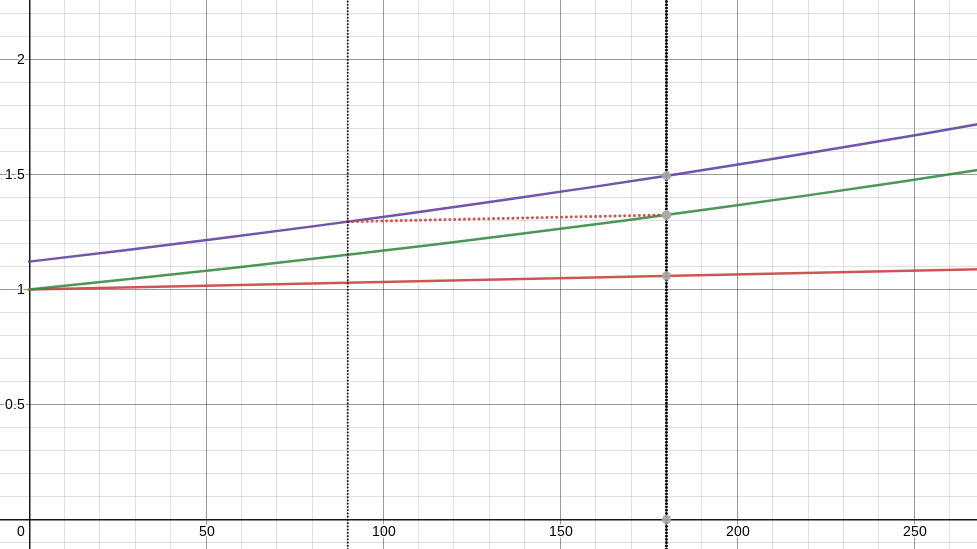
\includegraphics[width=\linewidth]{./ChickenBonds_Whitepaper_conservative_price.png}

The formula therefore for the conservative fair price is:

\begin{equation}
  \label{eq:conservative-1}
p_f(t) = p_r(t + T) - (n(t+T) - n(t))
\end{equation}

Where $n(t)$ represents the natural rate.

Assuming time $t$ to be denominated in days, the daily natural rate $r_m$ is expected to be low, so for values of $t$ in the order of magnitude of a year we can use the following approximation:

\begin{equation}
  \label{eq:conservative_natural_approximation}
n(t) = (1 + r_m)^t = 1 + r_m \cdot t
\end{equation}

We now seek a formula for $p_r$ which can in turn be used in $p_f$. 

\paragraph{With rebonding}
With rebonding this is quite hard, as we need the optimal rebonding time $T_{opt}$, which in itself uses the fair price (see \ref{sec:T_OP}).

If we assume that redemption price has an exponential behavior (due to the compounding effect of rebonding) of the form $p_r = a^t$ \footnote{This is probably wrong, as we will see in the no rebonding case!}, then fair price would be (using approximation in \ref{eq:conservative_natural_approximation}):

\begin{equation}
  \label{eq:conservative-2}
p_f(t) = a^{t+T} - r_m T
\end{equation}

Let’s try to find $a$.

For $t=0$, ${q_r}_0 = S_0$ and $p_r(0) = 1$. See \ref{sec:bootstrapping}.

Optimal rebonding time (using \ref{eq:optimal_chicken_in_1} and assuming $\alpha = 1$ to simplify):

\begin{equation}
  \label{eq:conservative_T_OP}
T_{opt} = \frac{1+ \sqrt{a^T - r_mT}}{a^T - r_mT - 1}
\end{equation}

The corresponding bTKN issuance expression for t = 0 is:

\begin{equation}
  \label{eq:conservative_issuance_proportion}
  \begin{split}
  \frac{T_{opt}}{T_{opt} + 1} & = \frac{\frac{1+ \sqrt{a^T - r_mT}}{a^T - r_mT - 1}}{\frac{1+ \sqrt{a^T - r_mT}}{a^T - r_mT - 1} + 1} \\
  & = \frac{1+ \sqrt{a^T - r_mT}}{1+ \sqrt{a^T - r_mT} + a^T - r_mT - 1} \\
  & = \frac{1+ \sqrt{a^T - r_mT}}{a^T - r_mT + \sqrt{a^T - r_mT}} \\
  & = \frac{(1+ \sqrt{a^T - r_mT})(a^T - r_mT - \sqrt{a^T - r_mT})}{(a^T - r_mT)^2 + a^T - r_mT} \\
  & = \frac{a^T - r_mT - \sqrt{a^T - r_mT} + (a^T - r_mT)\sqrt{a^T - r_mT} - (a^T - r_mT)}{(a^T - r_mT)(a^T - r_mT - 1)} \\
  & = \frac{- \sqrt{a^T - r_mT} + (a^T - r_mT)\sqrt{a^T - r_mT}}{(a^T - r_mT)(a^T - r_mT - 1)} \\
  & = \frac{(a^T - r_mT - 1)\sqrt{a^T - r_mT}}{(a^T - r_mT)(a^T - r_mT - 1)} \\
  & = \frac{\sqrt{a^T - r_mT}}{a^T - r_mT} \\
  & = \frac{1}{\sqrt{a^T - r_mT}}
  \end{split}
\end{equation}

Now moving forward to $t_1 = T_{opt}$:

\[
{q_p}_1 = {q_p}_0 \frac{a^T -r_mT}{\sqrt{a^T -r_mT}} = {q_p}_0 \sqrt{a^T - r_mT}
\]

\[
{q_r}_1 = {q_r}_0 + [({q_r}_0 + {q_p}_0)r_s + {q_d}_0 r_d] T_{opt} + {q_p}_0 \frac{1}{\sqrt{a^T - r_mT}}
\]

\[
S_1 = S_0 + \frac{{q_p}_0}{\sqrt{a^T - r_mT}} = {q_r}_0 + \frac{{q_p}_0}{\sqrt{a^T - r_mT}}
\]

So finally:

\begin{equation}
  \label{eq:conservative_p_r_1}
  \begin{split}
    {p_r}_1 & = \frac{{q_r}_1}{S_1} \\
    & = \frac{{q_r}_0 + [({q_r}_0 + {q_p}_0)r_s + {q_d}_0 r_d] T_{opt} + {q_p}_0 \frac{1}{\sqrt{a^T - r_mT}}}{{q_r}_0 + \frac{{q_p}_0}{\sqrt{a^T - r_mT}}} \\
    & = 1 + \frac{({q_r}_0 + {q_p}_0)r_s + {q_d}_0 r_d + {q_p}_0}{{q_r}_0 + \frac{{q_p}_0}{\sqrt{a^T - r_mT}}} \frac{1+ \sqrt{a^T - r_mT}}{a^T - r_mT - 1} \\
  \end{split}
\end{equation}

If we now equate this to $p_r(T_{opt})$ we get:
\begin{equation}
  \label{}
1 + \frac{({q_r}_0 + {q_p}_0)r_s + {q_d}_0 r_d + {q_p}_0}{{q_r}_0 + \frac{{q_p}_0}{\sqrt{a^T - r_mT}}} \frac{1+ \sqrt{a^T - r_mT}}{a^T - r_mT - 1} = a ^{\frac{1+ \sqrt{a^T - r_mT}}{a^T - r_mT - 1}}
\end{equation}

which seems quite hard to solve for $a$.

\paragraph{Without rebonding}

Although an approach without rebonding is unlikely to be fruitful since the redemption price will be too close to the natural rate, we can still try. Now we only account for the yield generated, which doesn’t increase the bTKN total supply:

\[
S_t = S_1 = S_0 = {q_r}_0
\]

We try to compute Reserve Bucket for several time intervals, let’s say daily:

\[
{q_r}_1 = {q_r}_0 + [({q_r}_0 + {q_p}_0) r_s + {q_d}_0 r_d] = {q_r}_0 + {q_r}_0 r_s + {q_p}_0 r_s + {q_d}_0 r_d
\]

\[
{q_r}_t = {q_r}_0(1+r_s)^t + ({q_p}_0 r_s + {q_d}_0 r_d) \left(r_s^t + \sum_{j=1}^{t-1} \binom{t}{j} a^j \right)
\]

So for time $t$ the redemption price would be:

\[
p_r(t) = \frac{{q_r}_t}{S_1} = \frac{{q_r}_0(1+r_s)^t + ({q_p}_0 r_s + {q_d}_0 r_d) \left(r_s^t + \sum_{j=1}^{t-1} \binom{t}{j} a^j \right)}{{q_r}_0}
\]

\begin{equation}
  \label{eq:conservative_p_r_base_2_a}
p_r(t) = (1+r_s)^t + \frac{{q_p}_0 r_s + {q_d}_0 r_d}{{q_r}_0} \left(r_s^{t-1} + \sum_{j=1}^{t-1} \binom{t}{j} r_s^{t-1-j} \right)
\end{equation}

We can approximate it to:

\begin{equation}
  \label{eq:conservative_p_r_base_2_b}
p_r(t) = (1+r_s)^t + \frac{{q_p}_0 r_s + {q_d}_0 r_d}{{q_r}_0} t
\end{equation}

In particular this shows that the assumption that redemption price follows a pure exponential $a^t$ is not correct.

\subsection{Self-reinforcing price impact}
It follows from equations \ref{eq:opt-rebonding-premium} that a higher premium $\lambda$ leads to a shorter rebonding period $t$ (the same is true for \ref{eq:optimal_chicken_in_2}, and for the break even time in \ref{eq:break_even_2}). As a consequence, we can expect bonders to chicken in earlier, resulting in a higher fraction of the bond $b_p$ that transitions into the Permanent Bucket, which makes the premium more sustainable and may be favorable for the fair price of bTKN (TODO: depends on the formula).

Thus, if the market price of bTKN increases while everything else stays equal, the chances are higher that the price will continue to rise in the future thanks to earlier chicken ins. While this effect may be not always be immediate, a large bTKN price hike could effectively push bonders beyond their optimal rebonding times.
Assuming perfectly rational behavior, this would result in immediate chicken ins (and rebonding).

TODO: check and update once we have a formula for the fair price

\subsection{Self-stabilizing effect of redemptions and its help to regain traction}
  \label{sec:self-stabilizing}
As redemptions reduce the Reserve Bucket and the bTKN supply in the same proportion, they indirectly increase the impact of the Permanent and the Pending Bucket on bTKN through a higher yield amplification. While the redemption price doesn't change when somebody redeems bTKN for TKN, the fair price and thus the expected premium grow as a result. 

We can therefore expect a self-stabilizing effect of redemptions: for any given $q_p \geq 0$ and $q_d > 0$ there should be an equilibrium state with $q_r > 0$ where $p_r = p_f$, making further redemptions and a complete drainage of the Reserve Bucket unlikely. Given this de facto lower bound on $q_r$, a portion of the Reserve Bucket will behave as if it was permanent.

Furthermore, natural fluctuations of the market price $p_m$ compared to $p_f$ could help the system regain traction should it ever reach a state where $p_f = p_r$: if the market temporarily prices the bTKN below its fair price ($p_m < p_f$), redemptions will kick in and raise $p_f$, increasing the odds that the market will return to $p_m > p_r$ and make bonding attractive again. This dynamic should apply even if $q_p = 0$, i.e. when bonding activity has come to a complete halt.

\section{Protocol enhancements and variations}
\subsection{Bootstrapping}
  \label{sec:bootstrapping}
Right after launch, the initial bTKN supply is 0 as the token is only minted upon chicken in events. Similarly, the Reserve Bucket is empty until the first bond holder chickens in. As a result, the redemption price $p_r$ (backing ratio) is undefined and cannot be used for calculating the accrued amount $s(t)$ during this bootstrapping period.

Meanwhile, the protocol is already earning yield on the Pending Bucket before anybody chickens in. Giving this yield to the bond holder who chickens ins first wouldn't seem fair. 

To tackle these problems, we can define the initial redemption price at the time of the first chicken in to be $p_r = 1$. The protocol thus needs to mint the same amount of bTKN as the amount of TKN acquired by the protocol on that first chicken in event. The accumulated yield of the Pending Bucket, which would normally belong to the Reserve Bucket, can be used to reward the LPs bootstrapping bTKN/TKN DEX pair (see \ref{sec:chicken-in-fee}).

\subsection{Two-bucket version}
\label{sec:two-bucket}
A Permanent Bucket may not be suitable for all use cases and protocol tokens. For example, if TKN is a token that is minted through loans, keeping a portion of it inside the Permanent Bucket forever would essentially reduce the circulating supply, which could impact the ability of borrowers to repay their debts. On the other hand, such tokens have usually no fixed or capped supply, but can be minted as needed, meaning that technically there's an unbounded amount of TKN that could be bonded over time.

This makes bonding more sustainable in the long run even without a Permanent Bucket.


\subsection{Automatically adjusting the steepness $\alpha$ of the accrual curve}
  \label{sec:adjustment}
The break even point (equation \ref{eq:break_even_2}) and the optimal rebonding time (equations \ref{eq:opt-rebonding-premium}, \ref{eq:optimal_chicken_in_2} and \ref{eq:optimal_chicken_in_2_fee}) heavily depend on the premium $\lambda$ as well as on $\alpha$, i.e. the steepness of the bTKN accrual curve $s(t)$. 

Simulations have shown that the premium $\lambda$ tends to decrease over time as the system matures. If  $\alpha$ was kept constant, this would mean that the break even and optimal rebonding times would increase throughout the lifetime of the system, making bonds less and less attractive due to a decreasing APR.

To avoid this outcome, the system could automatically adjust $\alpha$ to keep the optimal bonding duration constant. To that end, a controller could track the average (size-weighted) outstanding bond age and decrease $\alpha$ by a certain factor whenever the average age exceeds a given target age $T_a$. Assuming an even distribution of bond creation dates, we can deduce a target average chicken in time $T_t = 2T_a$.

\subsection{Redemption fee}
  \label{sec:redemption-fee}
To throttle the outflow of TKN from the Reserve Bucket, the system may charge a fee on redemptions, called the \textit{redemption fee}. The redeemer of $n$ bTKN would then get slightly less TKN than their pro rata share, i.e. $x < n \cdot p_r$. The difference $(n \cdot p_r - x)$ could be either kept in the Reserve Bucket or moved to the Permanent Bucket. 

In both cases, the captured fee increases the fair price by the same amount, in addition to the positive effect of the redemption as such on $p_f$ (see \ref{sec:self-stabilizing}). However, by leaving the fee in the Reserve Bucket the redemption price $p_r$ also increases, implying that by chickening in a user could directly impact the backing ratio and the cap of the existing users. To avoid such interference and potential bank run situations, it seems preferable to capture the fee revenue in the Permanent Bucket instead, resulting in a larger and more sustainable premium growth on top.  

An exponentially decaying fee schedule could be used to efficiently throttle redemptions: the fee is dynamically increased upon every redemption in function of the redeemed amount, decaying over time to a minimum when no redemptions take place.

\subsection{Chicken-in fee to incentivize bTKN/TKN LPs}
  \label{sec:chicken-in-fee}
Having a liquid bTKN/TKN market is crucial for bond holders to exit their positions or to rebond.
For that purpose, the system may incentivize LPs providing liquidity to a bTKN/TKN DEX pair by diverting a portion of the bonded amount upon every chicken-in. 

As a matter of fact, TKN and bTKN will be more strongly correlated in price than two random volatile assets, reducing the expected impermanent loss. The correlation between the two assets may influence the choice of the AMM, leaving room for custom trading curves optimized for lower slippage.

One way to fund the incentives is by charging a fee on the bTKN amount paid out upon a chicken in as described in \ref{sec:chicken-in}. 
Such an incentive scheme is dependent on the bonding activity and thus synchronized with the needs of the system and current bond holders wanting to exit.

\section{Conclusion}
Chicken Bonds will allow projects to bootstrap POL without having to pay for it. It achieves this by creating a flywheel effect between bonding and bTKN pricing: the more people bond, the more yield is retained for the bTKN holders. A higher yield in turn increases the price premium over the underlying TKN, making bonding more attractive through a higher APR. Meanwhile, the protocol is able to acquire both permanent and redeemable TKN liquidity, which can be put to different uses based on the needs of the project.


\end{document}
